%DIF 1c1-6
%DIF LATEXDIFF DIFFERENCE FILE
%DIF DEL toolkit-1p1-v5.tex   Sat Oct 31 09:01:57 2026
%DIF ADD toolkit-1p1-v6.tex   Sun Nov  1 10:29:52 2026
%DIF < \documentclass[prd,twocolumn,superscriptaddress,nofootinbib,amsmath,amssymb,floatfix]{revtex4-2}
%DIF -------
\documentclass[12pt]{iopart} %DIF > 
% amsmath after iopart: drop iopart's equation* so that amsmath can define it %DIF > 
\expandafter\let\csname equation*\endcsname\relax %DIF > 
\expandafter\let\csname endequation*\endcsname\relax %DIF > 
\usepackage{amsmath} %DIF > 
\usepackage{amssymb} %DIF > 
%DIF -------
\usepackage{graphicx}
\usepackage{xcolor}
\graphicspath{{../figs/}}
%DIF 5d10
%DIF < \usepackage{booktabs}
%DIF -------
\usepackage{tikz}
\usepackage[colorlinks=true,linkcolor=blue!50!black,citecolor=blue!50!black,urlcolor=blue!50!black]{hyperref}
\newcommand{\pending}[1]{\textcolor{red}{[#1]}}
\definecolor{bandA}{HTML}{008A7C}
\definecolor{bandB}{HTML}{C2610C}

%DIF < % 1+1 paper, split from counting-full-v2.tex (session 15, 2026-10-29). Companion: embedding-3p1-v1.tex; methodology: methodology-note-v1.tex.
%DIF -------
% 1+1 paper, split from counting-full-v2.tex (session 15, 2026-10-29). Companion: embedding-3p1-v*.tex; methodology: methodology-note-v*.tex. %DIF > 
%DIF < % Rules (Roberto): PRD register; failed attempts only in App. A (deletable); AI use = short disclosure + citation of the methodology note.
% Rules (Roberto): failed attempts only in App. B (deletable); AI use = short disclosure + citation of the methodology note. %DIF > 
%DIF < % Round 2 (referee agent): reframed as "exact identities and their deviations"; baseline table (r31); Laguerre vs fixed-n related fraction (r32);
% v2-v5: external referee rounds 1-4 (CQG track); history in the header of toolkit-1p1-v5.tex and in answers/answer-toolkit-1p1-v*.md. %DIF > 
%DIF < % propagator section moved before the embedding test; claims softened; qualifiers restored.
% v6 (session 21, 2026-11-01): IOP style for CQG (iopart.cls, IOP Publishing, LPPL; class files copied next to this source) and final language %DIF > 
%DIF < % v2 (session 17, external referee round 1, CQG track; answer in ~/Desktop/papers/1+1 CQG/answers/answer-toolkit-1p1-v2.md): restructured around
% pass. No change of content: every number, equation, claim, hedge and citation is as in v5. Style: \ack, Data availability statement, %DIF > 
%DIF < % Secs. III-IV; Laguerre target moved to Appendix A (Roberto); Table II with Hu-Meyer-Meyer and the bias-correction ablation (r36); curvature:
% IOP reference format, 'equation (n)', 'figure n', 'section n', roman d and e, tables with \br/\mr, -ize spellings (US, as v5 mostly used). %DIF > 
%DIF < % count-defined window, pooled estimator (the v1 offset was a ratio bias), sprinkled pairs, BD / chain-abundance noise (r37), FRW kernel (r38).
% Placeholder (\pending): Zenodo DOI (at submission). %DIF > 
%DIF < % Placeholders (\pending): Zenodo DOI (at submission). r27 filled in v4 (session 19).
%DIF < % v3 (session 18, external referee round 2, answer in ~/Desktop/papers/1+1 CQG/answers/answer-toolkit-1p1-v3.md): sprinkled-pair shortfall traced to
%DIF < % nearest-element selection (r40 select); order-only window in a causally convex region (r40 convex); FRW test with the pooled estimator (r40 frw);
%DIF < % noise in realistic use, P pairs in one diamond vs ordering fraction (r40 noise); kernel = first moment only; tau^4 systematic; refs; version refs removed.
%DIF < % v4 (session 19, external referee round 3, answer in ~/Desktop/papers/1+1 CQG/answers/answer-toolkit-1p1-v4.md): abstract matched to Sec. IV (in-region
%DIF < % bias, less precise than the ordering fraction); Mecke condition stated, count-defined example removed; one-region comparison rerun with a position-based
%DIF < % selection and a flat control at matched element count (r41); FRW shortfall 26-35 %; convexity argument without f, convexity as an assumption;
%DIF < % data availability worded as a commitment; Discussion: the curvature result is analytic and conceptual (optional locality test not run).
%DIF < % v5 (session 20, external referee round 4 = accept after 25-29; answer in ~/Desktop/papers/1+1 CQG/answers/answer-toolkit-1p1-v5.md): abstract
%DIF < % 'coefficients summed over the pairs of many sprinklings'; Fig. 3 cut stated (stricter than the fit window); flat-control lever arm; unrounded
%DIF < % inserted-pair offsets; N = 800 test: M, threshold, height context, small sample, full-test count 4/20 in Limitations; present tense; Last-Penrose cited.
%DIF PREAMBLE EXTENSION ADDED BY LATEXDIFF
%DIF UNDERLINE PREAMBLE %DIF PREAMBLE
\RequirePackage[normalem]{ulem} %DIF PREAMBLE
\RequirePackage{color}\definecolor{RED}{rgb}{1,0,0}\definecolor{BLUE}{rgb}{0,0,1} %DIF PREAMBLE
\providecommand{\DIFaddtex}[1]{{\protect\color{blue}\uwave{#1}}} %DIF PREAMBLE
\providecommand{\DIFdeltex}[1]{{\protect\color{red}\sout{#1}}} %DIF PREAMBLE
%DIF SAFE PREAMBLE %DIF PREAMBLE
\providecommand{\DIFaddbegin}{} %DIF PREAMBLE
\providecommand{\DIFaddend}{} %DIF PREAMBLE
\providecommand{\DIFdelbegin}{} %DIF PREAMBLE
\providecommand{\DIFdelend}{} %DIF PREAMBLE
\providecommand{\DIFmodbegin}{} %DIF PREAMBLE
\providecommand{\DIFmodend}{} %DIF PREAMBLE
%DIF FLOATSAFE PREAMBLE %DIF PREAMBLE
\providecommand{\DIFaddFL}[1]{\DIFadd{#1}} %DIF PREAMBLE
\providecommand{\DIFdelFL}[1]{\DIFdel{#1}} %DIF PREAMBLE
\providecommand{\DIFaddbeginFL}{} %DIF PREAMBLE
\providecommand{\DIFaddendFL}{} %DIF PREAMBLE
\providecommand{\DIFdelbeginFL}{} %DIF PREAMBLE
\providecommand{\DIFdelendFL}{} %DIF PREAMBLE
%DIF HYPERREF PREAMBLE %DIF PREAMBLE
\providecommand{\DIFadd}[1]{\texorpdfstring{\DIFaddtex{#1}}{#1}} %DIF PREAMBLE
\providecommand{\DIFdel}[1]{\texorpdfstring{\DIFdeltex{#1}}{}} %DIF PREAMBLE
\providecommand{\DIFscaledelfig}{0.5}
%DIF HIGHLIGHTGRAPHICS PREAMBLE %DIF PREAMBLE
\RequirePackage{settobox} %DIF PREAMBLE
\RequirePackage{letltxmacro} %DIF PREAMBLE
\newsavebox{\DIFdelgraphicsbox} %DIF PREAMBLE
\newlength{\DIFdelgraphicswidth} %DIF PREAMBLE
\newlength{\DIFdelgraphicsheight} %DIF PREAMBLE
% store original definition of \includegraphics %DIF PREAMBLE
\LetLtxMacro{\DIFOincludegraphics}{\includegraphics} %DIF PREAMBLE
\providecommand{\DIFaddincludegraphics}[2][]{{\color{blue}\fbox{\DIFOincludegraphics[#1]{#2}}}} %DIF PREAMBLE
\providecommand{\DIFdelincludegraphics}[2][]{% %DIF PREAMBLE
\sbox{\DIFdelgraphicsbox}{\DIFOincludegraphics[#1]{#2}}% %DIF PREAMBLE
\settoboxwidth{\DIFdelgraphicswidth}{\DIFdelgraphicsbox} %DIF PREAMBLE
\settoboxtotalheight{\DIFdelgraphicsheight}{\DIFdelgraphicsbox} %DIF PREAMBLE
\scalebox{\DIFscaledelfig}{% %DIF PREAMBLE
\parbox[b]{\DIFdelgraphicswidth}{\usebox{\DIFdelgraphicsbox}\\[-\baselineskip] \rule{\DIFdelgraphicswidth}{0em}}\llap{\resizebox{\DIFdelgraphicswidth}{\DIFdelgraphicsheight}{% %DIF PREAMBLE
\setlength{\unitlength}{\DIFdelgraphicswidth}% %DIF PREAMBLE
\begin{picture}(1,1)% %DIF PREAMBLE
\thicklines\linethickness{2pt} %DIF PREAMBLE
{\color[rgb]{1,0,0}\put(0,0){\framebox(1,1){}}}% %DIF PREAMBLE
{\color[rgb]{1,0,0}\put(0,0){\line( 1,1){1}}}% %DIF PREAMBLE
{\color[rgb]{1,0,0}\put(0,1){\line(1,-1){1}}}% %DIF PREAMBLE
\end{picture}% %DIF PREAMBLE
}\hspace*{3pt}}} %DIF PREAMBLE
} %DIF PREAMBLE
\LetLtxMacro{\DIFOaddbegin}{\DIFaddbegin} %DIF PREAMBLE
\LetLtxMacro{\DIFOaddend}{\DIFaddend} %DIF PREAMBLE
\LetLtxMacro{\DIFOdelbegin}{\DIFdelbegin} %DIF PREAMBLE
\LetLtxMacro{\DIFOdelend}{\DIFdelend} %DIF PREAMBLE
\DeclareRobustCommand{\DIFaddbegin}{\DIFOaddbegin \let\includegraphics\DIFaddincludegraphics} %DIF PREAMBLE
\DeclareRobustCommand{\DIFaddend}{\DIFOaddend \let\includegraphics\DIFOincludegraphics} %DIF PREAMBLE
\DeclareRobustCommand{\DIFdelbegin}{\DIFOdelbegin \let\includegraphics\DIFdelincludegraphics} %DIF PREAMBLE
\DeclareRobustCommand{\DIFdelend}{\DIFOaddend \let\includegraphics\DIFOincludegraphics} %DIF PREAMBLE
\LetLtxMacro{\DIFOaddbeginFL}{\DIFaddbeginFL} %DIF PREAMBLE
\LetLtxMacro{\DIFOaddendFL}{\DIFaddendFL} %DIF PREAMBLE
\LetLtxMacro{\DIFOdelbeginFL}{\DIFdelbeginFL} %DIF PREAMBLE
\LetLtxMacro{\DIFOdelendFL}{\DIFdelendFL} %DIF PREAMBLE
\DeclareRobustCommand{\DIFaddbeginFL}{\DIFOaddbeginFL \let\includegraphics\DIFaddincludegraphics} %DIF PREAMBLE
\DeclareRobustCommand{\DIFaddendFL}{\DIFOaddendFL \let\includegraphics\DIFOincludegraphics} %DIF PREAMBLE
\DeclareRobustCommand{\DIFdelbeginFL}{\DIFOdelbeginFL \let\includegraphics\DIFdelincludegraphics} %DIF PREAMBLE
\DeclareRobustCommand{\DIFdelendFL}{\DIFOaddendFL \let\includegraphics\DIFOincludegraphics} %DIF PREAMBLE
%DIF AMSMATHULEM PREAMBLE %DIF PREAMBLE
\makeatletter %DIF PREAMBLE
\let\sout@orig\sout %DIF PREAMBLE
\renewcommand{\sout}[1]{\ifmmode\text{\sout@orig{\ensuremath{#1}}}\else\sout@orig{#1}\fi} %DIF PREAMBLE
\makeatother %DIF PREAMBLE
%DIF END PREAMBLE EXTENSION ADDED BY LATEXDIFF

\begin{document}

\DIFdelbegin %DIFDELCMD < \title{%%%
\DIFdelend \DIFaddbegin \title[Spatial distance and curvature from a counting identity]{\DIFaddend Spatial distance and curvature from an exact counting identity in two-dimensional causal sets}

\author{Roberto Bada\DIFaddbegin \DIFadd{$^{1,2}$}\DIFaddend }
\DIFdelbegin %DIFDELCMD < \email{roberto@sapereia.com}
%DIFDELCMD < \affiliation{SapereIA, Barcelona, Spain}
%DIFDELCMD < \affiliation{Institute of Cosmos Sciences, University of Barcelona (ICCUB), Barcelona, Spain}
%DIFDELCMD < %%%
\DIFdelend 

\DIFdelbegin %DIFDELCMD < \date{\today}
%DIFDELCMD < %%%
\DIFdelend \DIFaddbegin \address{$^1$ SapereIA, Barcelona, Spain}
\address{$^2$ Institute of Cosmos Sciences, University of Barcelona (ICCUB), Barcelona, Spain}
\ead{roberto@sapereia.com}
\DIFaddend 

\begin{abstract}
In causal set theory, geometry must be recovered from the causal order and from counting. In two dimensions, the causal-overlap regions of Bogu\~n\'a and Krioukov satisfy an exact identity: for two spacelike elements and \emph{any} element $c$ in their common past, $d^2=2V_AV_B/V_C$ in flat spacetime. With a Poisson bias correction\DIFdelbegin \DIFdel{it }\DIFdelend \DIFaddbegin \DIFadd{, the identity }\DIFaddend gives a spatial-distance estimator that is unbiased for $d^2$ above two discreteness lengths. On the same pairs\DIFdelbegin \DIFdel{it }\DIFdelend \DIFaddbegin \DIFadd{, this estimator }\DIFaddend is more accurate than the equal-depth construction of Bogu\~n\'a and Krioukov at all separations, \DIFaddbegin \DIFadd{and }\DIFaddend the freedom in the choice of $c$ \DIFdelbegin \DIFdel{being }\DIFdelend \DIFaddbegin \DIFadd{is }\DIFaddend what improves on it\DIFdelbegin \DIFdel{; between }\DIFdelend \DIFaddbegin \DIFadd{. Between }\DIFaddend two and ten discreteness lengths it is as accurate as\DIFaddbegin \DIFadd{, }\DIFaddend or more accurate than\DIFaddbegin \DIFadd{, }\DIFaddend the past--future construction of Hu, Meyer and Meyer, which is more accurate at larger separations. In curved spacetime the identity fails in a way that depends on the depth of $c$. In de Sitter space $d^2_{\rm est}/d^2=\tanh^2(H\tau/2)/[2\ln\cosh(H\tau/2)]=1-R\tau^2/16+O(\tau^4)$, and in any $1+1$ FRW spacetime, to leading order in the depth, the failure measures the scalar curvature one third of the way from the pair to $c$. A fit of this depth drift, with its coefficients summed over the pairs of many independent sprinklings, reproduces the same fit on the exact continuum volumes\DIFdelbegin \DIFdel{, }\DIFdelend \DIFaddbegin \DIFadd{. It does so }\DIFaddend for pairs inserted by hand (de Sitter, flat and FRW sprinklings) and for all sprinkled pairs of a position-based selection (de Sitter and flat, within $1.7\sigma$); selecting the elements nearest to given points biases it low. On a sprinkling of a causally convex region, such as an interval of the causal set, \DIFdelbegin \DIFdel{its }\DIFdelend \DIFaddbegin \DIFadd{the fit }\DIFaddend window needs no coordinates. For the curvature of a given region, however, \DIFdelbegin \DIFdel{it }\DIFdelend \DIFaddbegin \DIFadd{the fit }\DIFaddend is less precise than the ordering fraction (in de Sitter space its spread between sprinklings is about three times larger) and, within one region, biased low. As a supporting diagnostic\DIFaddbegin \DIFadd{, }\DIFaddend we calibrate the Lorentzian-embedding test of Clough and Evans and add the fraction of null-separated pairs, which lets the test reject layered orders on its own. \DIFdelbegin \DIFdel{A }\DIFdelend \DIFaddbegin \DIFadd{An appendix gives a }\DIFaddend Laguerre identity for the mean of Johnston's propagator at fixed interval size\DIFdelbegin \DIFdel{is given in an appendix}\DIFdelend .
\end{abstract}

\DIFaddbegin \vspace{2pc}
\noindent{\it Keywords\/}\DIFadd{: causal sets, two-dimensional orders, spatial distance, scalar curvature, de Sitter space, Lorentzian embedding
}

\submitto{\CQG}

\DIFaddend \maketitle

\section{Introduction}\label{sec:intro}
A causal set is a locally finite partially ordered set: every interval $I(x,y)=\{z:x\prec z\prec y\}$ is finite~\cite{BLMS87,Surya19}. Causal set theory proposes that spacetime is such a set, with the continuum emerging at large scales. The number of elements in a region then measures its spacetime volume\DIFaddbegin \DIFadd{, }\DIFaddend and the order fixes the light cones\DIFdelbegin \DIFdel{; the kinematic programme }\DIFdelend \DIFaddbegin \DIFadd{. The kinematic program }\DIFaddend is to recover all other geometric information from these two ingredients.

Part of this program\DIFdelbegin \DIFdel{me}\DIFdelend  is well established. The longest chain between two elements estimates their proper time~\cite{BrightwellGregory91}; interval and chain abundances give the dimension~\cite{Myrheim78,Meyer88} and the curvature~\cite{RSS13,GlaserSurya13}; \DIFaddbegin \DIFadd{and }\DIFaddend the Benincasa--Dowker operator gives the scalar curvature and the action~\cite{BD10,DowkerGlaser13}. Spatial distance is harder, because spacelike elements bound no interval. Bogu\~n\'a and Krioukov measured it through the overlap of the pasts of two elements\DIFaddbegin \DIFadd{, }\DIFaddend as seen from an element $c$ at equal proper time below both~\cite{BK24}\DIFdelbegin \DIFdel{; }\DIFdelend \DIFaddbegin \DIFadd{. }\DIFaddend Brightwell and Gregory\DIFaddbegin \DIFadd{, }\DIFaddend and Rideout and Wallden\DIFaddbegin \DIFadd{, }\DIFaddend used the smallest interval containing both elements~\cite{BrightwellGregory91,RideoutWallden09}\DIFdelbegin \DIFdel{; }\DIFdelend \DIFaddbegin \DIFadd{. }\DIFaddend Hu, Meyer and Meyer gave an exact reconstruction in $1+1$ dimensions from a past and a future element~\cite{HMM25}. Whether a causal set resembles a manifold at all is tested by dimension estimators, interval abundances~\cite{GlaserSurya13} and Lorentzian embeddings~\cite{CloughEvans16,Henson06,Johnston25}. Matter can be introduced through Johnston's sum over chains~\cite{Johnston08,Johnston09}, whose average over sprinklings reproduces the Klein--Gordon propagator.

Two-dimensional causal sets are a natural laboratory\DIFdelbegin \DIFdel{: every }\DIFdelend \DIFaddbegin \DIFadd{. Every }\DIFaddend $1+1$ metric is conformally flat, intervals are rectangles in light-cone coordinates, and a sprinkled diamond is a uniformly random two-dimensional order, whose combinatorics is known~\cite{BHS08,Surya12}; the \DIFdelbegin \DIFdel{$e^{-\beta S}$ }\DIFdelend \DIFaddbegin \DIFadd{$\rme^{-\beta S}$ }\DIFaddend model of two-dimensional orders also has a well-studied phase structure~\cite{BHS08,Surya12,GOS18}. This paper is built on one exact identity that follows from these facts, and on the use of its violation as a measure of curvature. The \emph{rectangle identity} expresses the spatial distance of two elements through the overlap volumes seen from any element of their common past (\DIFdelbegin \DIFdel{Sec.}\DIFdelend \DIFaddbegin \DIFadd{section}\DIFaddend ~\ref{sec:dist}). It removes the equal-depth requirement of\DIFdelbegin \DIFdel{Ref.}\DIFdelend ~\cite{BK24} and yields a distance estimator, which we compare with the equal-depth, past--future and Hu--Meyer--Meyer constructions on the same pairs. In curved spacetime the identity fails as a function of the depth of $c$\DIFdelbegin \DIFdel{; we }\DIFdelend \DIFaddbegin \DIFadd{. We }\DIFaddend derive this depth drift in closed form in de Sitter space and to leading order in any $1+1$ FRW spacetime, and turn it into a curvature estimator (\DIFdelbegin \DIFdel{Sec.}\DIFdelend \DIFaddbegin \DIFadd{section}\DIFaddend ~\ref{sec:curv}). Spatial distance in causal sets has also been approached through thickened antichains and induced distances on spatial hypersurfaces~\cite{MRS06,MRS07,ESV19}\DIFdelbegin \DIFdel{, and curvature through }\DIFdelend \DIFaddbegin \DIFadd{. Curvature has also been obtained from }\DIFaddend interval and chain abundances in small causal diamonds~\cite{RSS13,KhetrapalSurya13} and \DIFaddbegin \DIFadd{from }\DIFaddend the Benincasa--Dowker operator~\cite{BD10}; we compare \DIFaddbegin \DIFadd{our curvature estimator }\DIFaddend with the last two at equal density.

As a supporting diagnostic\DIFaddbegin \DIFadd{, }\DIFaddend we calibrate the Lorentzian-embedding test of Clough and Evans and add a statistic that lets it reject layered orders on its own (\DIFdelbegin \DIFdel{Sec.}\DIFdelend \DIFaddbegin \DIFadd{section}\DIFaddend ~\ref{sec:embed})\DIFdelbegin \DIFdel{, and }\DIFdelend \DIFaddbegin \DIFadd{. We }\DIFaddend apply it to sequential growth and to configurations of the \DIFdelbegin \DIFdel{$e^{-\beta S}$ model (Sec.}\DIFdelend \DIFaddbegin \DIFadd{$\rme^{-\beta S}$ model (section}\DIFaddend ~\ref{sec:phases}). Section~\ref{sec:disc} discusses novelty and limitations. \DIFdelbegin \DIFdel{Appendix~}\DIFdelend \ref{app:prop} gives a combinatorial identity for Johnston's propagator at fixed interval size, and \DIFdelbegin \DIFdel{Appendix~}\DIFdelend \ref{app:dropped} summarizes other approaches we tested. Spatial distances in $3+1$ dimensions, where the rectangle identity has no analogue, are treated in a companion paper~\cite{Embedding}.

\section{Setting}\label{sec:setting}
Test causal sets are generated by sprinkling: a Poisson process of density $\rho$ in a region of a given spacetime, with the order induced by the light cones. The coordinates are then discarded and used only for comparison. We write $\ell=\rho^{-1/2}$ for the discreteness length: a region of volume $\ell^2$ contains one element on average.

We use light-cone coordinates $u=t-x$, $v=t+x$, in which \DIFdelbegin \DIFdel{$dt\,dx=du\,dv/2$ }\DIFdelend \DIFaddbegin \DIFadd{$\rmd t\,\rmd x=\rmd u\,\rmd v/2$, }\DIFaddend and $x\prec y$ if and only if $u_x<u_y$ and $v_x<v_y$. The interval between $x\prec y$ is the rectangle $[u_x,u_y]\times[v_x,v_y]$, with volume $V=\Delta u\,\Delta v/2=\tau^2/2$. A sprinkled causal diamond is therefore a uniformly random two-dimensional order, the intersection of two random linear orders~\cite{BHS08,Surya12}. For two spacelike elements, $d^2=\Delta x^2-\Delta t^2=-\Delta u\,\Delta v$.

The proper time \DIFaddbegin \DIFadd{obtained }\DIFaddend from the longest chain has mean $\simeq2\sqrt n$ in an interval of $n$ elements, with Tracy--Widom fluctuations of order $n^{1/6}$~\cite{BDJ99}\DIFdelbegin \DIFdel{; wherever }\DIFdelend \DIFaddbegin \DIFadd{. Wherever }\DIFaddend a volume is available\DIFaddbegin \DIFadd{, }\DIFaddend we use the count instead\DIFdelbegin \DIFdel{, }\DIFdelend \DIFaddbegin \DIFadd{: }\DIFaddend $\tau^2=2n/\rho$. Pairs of elements in one sprinkling share elements\DIFdelbegin \DIFdel{and }\DIFdelend \DIFaddbegin \DIFadd{, so }\DIFaddend their errors are correlated; quoted uncertainties are therefore computed from the spread between independent sprinklings.

\section{The rectangle identity and a distance estimator}\label{sec:dist}
Let $a,b$ be spacelike and \DIFaddbegin \DIFadd{let }\DIFaddend $c$ \DIFaddbegin \DIFadd{be }\DIFaddend an element in their common past. Following\DIFdelbegin \DIFdel{Ref.}\DIFdelend ~\cite{BK24}, we split the two intervals into
\begin{equation}
\DIFdelbegin %DIFDELCMD < \begin{gathered}
%DIFDELCMD < A=I(c,a)\setminus I(c,b),\qquad B=I(c,b)\setminus I(c,a),\\
%DIFDELCMD < C=I(c,a)\cap I(c,b).
%DIFDELCMD < \end{gathered}
%DIFDELCMD < %%%
\DIFdelend \DIFaddbegin \DIFadd{A=I(c,a)\setminus I(c,b),\qquad B=I(c,b)\setminus I(c,a),\qquad
C=I(c,a)\cap I(c,b).
}\DIFaddend \end{equation}
Bogu\~n\'a and Krioukov choose $c$ at equal proper time below $a$ and $b$\DIFaddbegin \DIFadd{, }\DIFaddend and derive $d$ from the overlap fraction. In $1+1$ dimensions the choice of $c$ is immaterial, because of the following identity (\DIFdelbegin \DIFdel{Fig.}\DIFdelend \DIFaddbegin \DIFadd{figure}\DIFaddend ~\ref{fig:tiles}).

\begin{figure}[t]
\centering
\DIFdelbeginFL %DIFDELCMD < \begin{tikzpicture}[scale=0.72]
%DIFDELCMD <   \fill[bandA!25] (0,0) rectangle (1.6,1.3);
%DIFDELCMD <   \fill[bandB!25] (0,1.3) rectangle (1.6,4);
%DIFDELCMD <   \fill[bandB!25] (1.6,0) rectangle (4.2,1.3);
%DIFDELCMD <   \fill[gray!25] (1.6,1.3) rectangle (4.2,4);
%DIFDELCMD <   \draw[thick] (0,0) rectangle (4.2,4);
%DIFDELCMD <   \draw (1.6,0) -- (1.6,4); \draw (0,1.3) -- (4.2,1.3);
%DIFDELCMD <   \node at (0.8,0.65) {$C$}; \node at (0.8,2.65) {$A$}; \node at (2.9,0.65) {$B$}; \node at (2.9,2.65) {$D$};
%DIFDELCMD <   \fill (0,0) circle (2pt) node[below left] {$c$};
%DIFDELCMD <   \fill (1.6,4) circle (2pt) node[above] {$a$};
%DIFDELCMD <   \fill (4.2,1.3) circle (2pt) node[right] {$b$};
%DIFDELCMD <   \fill (4.2,4) circle (2pt) node[above right] {join};
%DIFDELCMD <   \draw[->,gray] (-0.3,-0.3) -- (4.8,-0.3) node[right] {$u$};
%DIFDELCMD <   \draw[->,gray] (-0.3,-0.3) -- (-0.3,4.6) node[above] {$v$};
%DIFDELCMD < \end{tikzpicture}
%DIFDELCMD < %%%
\DIFdelendFL \DIFaddbeginFL \begin{tikzpicture}[scale=0.8]
  \fill[bandA!25] (0,0) rectangle (1.6,1.3);
  \fill[bandB!25] (0,1.3) rectangle (1.6,4);
  \fill[bandB!25] (1.6,0) rectangle (4.2,1.3);
  \fill[gray!25] (1.6,1.3) rectangle (4.2,4);
  \draw[thick] (0,0) rectangle (4.2,4);
  \draw (1.6,0) -- (1.6,4); \draw (0,1.3) -- (4.2,1.3);
  \node at (0.8,0.65) {$C$}; \node at (0.8,2.65) {$A$}; \node at (2.9,0.65) {$B$}; \node at (2.9,2.65) {$D$};
  \fill (0,0) circle (2pt) node[below left] {$c$};
  \fill (1.6,4) circle (2pt) node[above] {$a$};
  \fill (4.2,1.3) circle (2pt) node[right] {$b$};
  \fill (4.2,4) circle (2pt) node[above right] {join};
  \draw[->,gray] (-0.3,-0.3) -- (4.8,-0.3) node[right] {$u$};
  \draw[->,gray] (-0.3,-0.3) -- (-0.3,4.6) node[above] {$v$};
\end{tikzpicture}
\DIFaddendFL \caption{The rectangle identity in light-cone coordinates (rotated by $45^\circ$ with respect to the usual picture). The rectangle from $c$ to the join of $a$ and $b$ splits into the overlap $C$, the strips $A$ and $B$\DIFaddbeginFL \DIFaddFL{, each }\DIFaddendFL seen by only one of \DIFdelbeginFL \DIFdelFL{$a,b$}\DIFdelendFL \DIFaddbeginFL \DIFaddFL{$a$ and $b$}\DIFaddendFL , and the tile $D$\DIFdelbeginFL \DIFdelFL{with }\DIFdelendFL \DIFaddbeginFL \DIFaddFL{, which has }\DIFaddendFL $a$ and $b$ at opposite corners. Opposite tiles have equal products, $V_CV_D=V_AV_B$, and $V_D=d^2/2$.}
\label{fig:tiles}
\end{figure}

\emph{Derivation.} Place $c$ at the origin and take $u_a<u_b$ \DIFdelbegin \DIFdel{, }\DIFdelend \DIFaddbegin \DIFadd{and }\DIFaddend $v_a>v_b$ ($a$ and $b$ spacelike). Then $I(c,a)=[0,u_a]\times[0,v_a]$ and $I(c,b)=[0,u_b]\times[0,v_b]$. The rectangle from $c$ to the join $(u_b,v_a)$ splits into four tiles,
\begin{equation}
\begin{aligned}
C&=[0,u_a]\times[0,v_b], & A&=[0,u_a]\times[v_b,v_a],\\
B&=[u_a,u_b]\times[0,v_b], & D&=[u_a,u_b]\times[v_b,v_a].
\end{aligned}
\end{equation}
With $\Delta u=u_b-u_a$ and $\Delta v=v_a-v_b$, the volumes are $V_C=u_av_b/2$, $V_A=u_a\Delta v/2$, $V_B=\Delta u\,v_b/2$ \DIFdelbegin \DIFdel{, }\DIFdelend \DIFaddbegin \DIFadd{and }\DIFaddend $V_D=\Delta u\,\Delta v/2$, so that $V_CV_D=V_AV_B$. The tile $D$ has $a$ and $b$ at opposite corners, so $V_D=d^2/2$. Hence, for every $c$ in the common past,
\begin{equation}
d^2=\frac{2V_AV_B}{V_C}.
\label{eq:rect}
\end{equation}
The tile $D$ is the interval between the meet and the join of $a$ and $b$, i.e.\DIFdelbegin \DIFdel{, }\DIFdelend \DIFaddbegin \DIFadd{\ }\DIFaddend the region whose volume defines the $1+1$ spatial distance of Brightwell and Gregory and of Rideout and Wallden~\cite{BrightwellGregory91,RideoutWallden09}. The identity shows that this volume can be read from the past alone, through a single element $c$. The equal-time choice of\DIFdelbegin \DIFdel{Ref.~\mbox{%DIFAUXCMD
\cite{BK24} }\hskip0pt%DIFAUXCMD
is }\DIFdelend \DIFaddbegin \DIFadd{~\mbox{%DIFAUXCMD
\cite{BK24} }\hskip0pt%DIFAUXCMD
corresponds to }\DIFaddend $V_A=V_B$, in which case their $1+1$ formula reduces to \DIFdelbegin \DIFdel{Eq.~\eqref{eq:rect}; for }\DIFdelend \DIFaddbegin \DIFadd{equation~}\eref{eq:rect}\DIFadd{. For }\DIFaddend general $c$\DIFaddbegin \DIFadd{, }\DIFaddend the search for equal-time elements, which requires the density and the dimension, is unnecessary. The identity relies on the overlap of two $1+1$ intervals being again an interval\DIFdelbegin \DIFdel{; in }\DIFdelend \DIFaddbegin \DIFadd{. In }\DIFaddend higher dimensions it is not, and \DIFdelbegin \DIFdel{Eq.~\eqref{eq:rect} }\DIFdelend \DIFaddbegin \DIFadd{equation~}\eref{eq:rect} \DIFaddend has no direct analogue.

\emph{Estimator.} On a causal set, $V_X$ is replaced by $N_X/\rho$, \DIFaddbegin \DIFadd{where $N_X$ is }\DIFaddend the number of elements in the region \DIFaddbegin \DIFadd{$X$}\DIFaddend . The three regions are disjoint, so $N_A$, $N_B$ \DIFdelbegin \DIFdel{, }\DIFdelend \DIFaddbegin \DIFadd{and }\DIFaddend $N_C$ are independent Poisson variables with means $\lambda_X=\rho V_X$. The product $N_AN_B$ is unbiased for $\lambda_A\lambda_B$, but $1/N_C$ is biased and \DIFaddbegin \DIFadd{is }\DIFaddend undefined at $N_C=0$. Since \DIFdelbegin \DIFdel{$E[1/(N+1)]=(1-e^{-\lambda})/\lambda$ }\DIFdelend \DIFaddbegin \DIFadd{$E[1/(N+1)]=(1-\rme^{-\lambda})/\lambda$ }\DIFaddend for a Poisson variable \DIFaddbegin \DIFadd{$N$ with mean $\lambda$}\DIFaddend ,
\begin{equation}
\widehat{d^2}=\frac{2N_AN_B}{\rho\,(N_C+1)}
\label{eq:est}
\end{equation}
is unbiased for $d^2$ up to a factor \DIFdelbegin \DIFdel{$1-e^{-\lambda_C}$}\DIFdelend \DIFaddbegin \DIFadd{$1-\rme^{-\lambda_C}$}\DIFaddend . The relative variance is approximately $1/\lambda_A+1/\lambda_B+1/\lambda_C$, so the deepest available $c$ is optimal\DIFdelbegin \DIFdel{; }\DIFdelend \DIFaddbegin \DIFadd{, and }\DIFaddend we take the element with the largest $N_C$. The strips $A$ and $B$ are long and thin and contain many elements even when $d\sim\ell$\DIFdelbegin \DIFdel{, which }\DIFdelend \DIFaddbegin \DIFadd{; this }\DIFaddend is why the estimator works down to the discreteness scale\DIFdelbegin \DIFdel{; by }\DIFdelend \DIFaddbegin \DIFadd{. By }\DIFaddend contrast, a direct count of the tile $D$ has relative variance $1/\lambda_D=2\ell^2/d^2$, which is $\tfrac12$ at $d=2\ell$.

\emph{Tests.} \DIFdelbegin \DIFdel{Two pair selectionsare used, and the difference matters for the }\DIFdelend \DIFaddbegin \DIFadd{We use two pair selections, which differ in the }\DIFaddend size of the errors\DIFdelbegin \DIFdel{: }\DIFdelend \DIFaddbegin \DIFadd{. }\DIFaddend Table~\ref{tab:dist} and \DIFdelbegin \DIFdel{Fig.}\DIFdelend \DIFaddbegin \DIFadd{figure}\DIFaddend ~\ref{fig:distance} use random spacelike pairs among \emph{late} elements of flat sprinklings of a unit diamond\DIFdelbegin \DIFdel{, which }\DIFdelend \DIFaddbegin \DIFadd{; these pairs }\DIFaddend have large common pasts\DIFdelbegin \DIFdel{; }\DIFdelend \DIFaddbegin \DIFadd{. }\DIFaddend Table~\ref{tab:base} uses pairs in the \emph{middle} of the diamond, which have both a common past and a common future\DIFaddbegin \DIFadd{, }\DIFaddend but smaller ones. In both \DIFaddbegin \DIFadd{cases}\DIFaddend , $c$ is the deepest element for each pair. The median error falls approximately as $N^{-1/2}$ at large $d$\DIFdelbegin \DIFdel{, and remains at $15$--$25\%$ below }\DIFdelend \DIFaddbegin \DIFadd{. Below }\DIFaddend $2\ell$, the discreteness scale itself, \DIFdelbegin \DIFdel{where }\DIFdelend \DIFaddbegin \DIFadd{it remains at $15$--$25\%$, and }\DIFaddend $\widehat{d^2}$ is also biased high \DIFaddbegin \DIFadd{there }\DIFaddend [by $(37\pm7)\%$ at $N=4000$ on the pairs of \DIFdelbegin \DIFdel{Table}\DIFdelend \DIFaddbegin \DIFadd{table}\DIFaddend ~\ref{tab:base}].
\DIFaddbegin 

\DIFaddend Table~\ref{tab:base} compares the estimator with the existing constructions on the same pairs: the equal-depth filter of Bogu\~n\'a and Krioukov [\DIFdelbegin \DIFdel{their Eq.}\DIFdelend \DIFaddbegin \DIFadd{equation}\DIFaddend ~(34) \DIFaddbegin \DIFadd{of~\mbox{%DIFAUXCMD
\cite{BK24}}\hskip0pt%DIFAUXCMD
}\DIFaddend ]; the smallest interval $I(c,f)$ with $c\prec a,b\prec f$ (Brightwell--Gregory, Rideout--Wallden), $d^2=2(N_{\min}-2)/\rho$; and the construction of Hu, Meyer and Meyer~\cite{HMM25}\DIFdelbegin \DIFdel{, who }\DIFdelend \DIFaddbegin \DIFadd{. They }\DIFaddend showed that for $p\prec a,b\prec q$ with all four proper times equal to $s$, $d^2=\tau_{pq}^2-4s^2$\DIFdelbegin \DIFdel{. They gave it }\DIFdelend \DIFaddbegin \DIFadd{, and gave this }\DIFaddend as an exact statement about Minkowski space\DIFdelbegin \DIFdel{; on }\DIFdelend \DIFaddbegin \DIFadd{. On }\DIFaddend the causal set\DIFaddbegin \DIFadd{, }\DIFaddend we read every $\tau^2$ from a count ($\tau^2=2N/\rho$), take $p$ from the common past and $q$ from the common future, \DIFaddbegin \DIFadd{and }\DIFaddend keep the pairs $(p,q)$ whose four counts agree within Poisson noise ($\chi^2<3$)\DIFdelbegin \DIFdel{, and among them use the one }\DIFdelend \DIFaddbegin \DIFadd{. Among these we use the pair }\DIFaddend with the smallest counts, which has the smallest variance\DIFdelbegin \DIFdel{(}\DIFdelend \DIFaddbegin \DIFadd{; }\DIFaddend choosing instead the best-matched \DIFaddbegin \DIFadd{pair, }\DIFaddend or averaging over all matched pairs\DIFaddbegin \DIFadd{, }\DIFaddend is less accurate\DIFdelbegin \DIFdel{)}\DIFdelend . Two ablations separate the ingredients of our estimator: the same deepest $c$ without the Poisson correction, \DIFdelbegin \DIFdel{$2N_AN_B/\rho N_C$}\DIFdelend \DIFaddbegin \DIFadd{$2N_AN_B/(\rho N_C)$}\DIFaddend , and the equal-depth elements $c$ of\DIFdelbegin \DIFdel{Ref.}\DIFdelend ~\cite{BK24} with the corrected formula, \DIFdelbegin \DIFdel{Eq.~\eqref{eq:est}}\DIFdelend \DIFaddbegin \DIFadd{equation~}\eref{eq:est}\DIFaddend .

Above $2\ell$ the rectangle estimator is unbiased for $d^2$ within the uncertainties. Between $2\ell$ and $10\ell$ its median error is the smallest\DIFdelbegin \DIFdel{; the }\DIFdelend \DIFaddbegin \DIFadd{. The }\DIFaddend Hu--Meyer--Meyer estimate is close in error but biased high by about $20\%$, because $\tau_{pq}^2-4s^2$ is a small difference of two noisy terms. Above $10\ell$ the Hu--Meyer--Meyer estimate is unbiased and the most accurate, with half the error of ours or less\DIFdelbegin \DIFdel{: there }\DIFdelend \DIFaddbegin \DIFadd{. There }\DIFaddend the tile between $a$ and $b$ is large, and a direct count of it, corrected exactly by the four equal intervals, beats reading the same volume from the strips. For $d$ itself the rectangle estimator reads $1$--$3.5\%$ low, as expected from the square root of an unbiased estimate of $d^2$. The plain past--future count is biased high, because the smallest interval between elements cannot coincide with the tile $D$.
\DIFaddbegin 

\DIFaddend The ablations locate the gain over the equal-depth estimator. With the deepest $c$, $N_C$ is large and the Poisson correction makes no difference. With the equal-depth elements, where $N_C$ is small, the correction removes the bias of the equal-depth estimator ($+10\%\to+1\%$ and $+6\%\to+2\%$ between $2\ell$ and $10\ell$) \DIFdelbegin \DIFdel{, }\DIFdelend but not its larger error ($0.129$ and $0.104$, against $0.095$ and $0.059$ with the deepest $c$). The bias of\DIFdelbegin \DIFdel{Ref.}\DIFdelend ~\cite{BK24} on the causal set thus comes from the uncorrected ratio of small counts, and the \DIFdelbegin \DIFdel{accuracy gain }\DIFdelend \DIFaddbegin \DIFadd{gain in accuracy comes }\DIFaddend from the freedom to use the deepest $c$, which the identity provides. The equal-depth filter also returns no estimate for $10$--$30\%$ of the pairs. Below $2\ell$ every estimator is poor, and the two past--future constructions fail entirely (median errors above $50\%$). For the baseline tests we add a bottom element that precedes all others\DIFdelbegin \DIFdel{; the }\DIFdelend \DIFaddbegin \DIFadd{. The }\DIFaddend deepest $c$ is then always that element\DIFdelbegin \DIFdel{, }\DIFdelend \DIFaddbegin \DIFadd{; it is }\DIFaddend selected without reference to its own count, so the selection introduces no bias\DIFdelbegin \DIFdel{(in Table}\DIFdelend \DIFaddbegin \DIFadd{. (In table}\DIFaddend ~\ref{tab:dist}, \DIFdelbegin \DIFdel{without such an element, it }\DIFdelend \DIFaddbegin \DIFadd{which has no such element, the deepest $c$ }\DIFaddend is one of the lowest elements\DIFdelbegin \DIFdel{); the }\DIFdelend \DIFaddbegin \DIFadd{.) The }\DIFaddend freedom in the choice of $c$ is exercised by the curvature tests of \DIFdelbegin \DIFdel{Sec.}\DIFdelend \DIFaddbegin \DIFadd{section}\DIFaddend ~\ref{sec:curv}.

\begin{table}[t]
\caption{\DIFaddbeginFL \label{tab:dist}\DIFaddendFL Median relative error of \DIFdelbeginFL \DIFdelFL{Eq.}\DIFdelendFL \DIFaddbeginFL \DIFaddFL{equation}\DIFaddendFL ~\DIFdelbeginFL \DIFdelFL{\eqref{eq:est} }\DIFdelendFL \DIFaddbeginFL \eref{eq:est} \DIFaddendFL with the deepest $c$; flat $1+1$ sprinklings, 300 pairs among late elements in each of 4 sprinklings per $N$. (Table~\ref{tab:base} uses pairs in the middle of the diamond, with smaller common pasts, and therefore \DIFaddbeginFL \DIFaddFL{has }\DIFaddendFL larger errors.)}
\DIFdelbeginFL %DIFDELCMD < \label{tab:dist}
%DIFDELCMD < \begin{ruledtabular}
%DIFDELCMD < \begin{tabular}{rccc}
%DIFDELCMD < $N$ & $d<2\ell$ & $2\ell$--$10\ell$ & $>10\ell$\\
%DIFDELCMD < \hline
%DIFDELCMD < 1000 & 23\% & 6.5\% & 5.2\%\\
%DIFDELCMD < 2000 & 15\% & 5.0\% & 3.4\%\\
%DIFDELCMD < 4000 & 19\% & 5.1\% & 2.5\%\\
%DIFDELCMD < \end{tabular}
%DIFDELCMD < \end{ruledtabular}
%DIFDELCMD < %%%
\DIFdelendFL \DIFaddbeginFL \begin{indented}
\item[]\begin{tabular}{@{}rccc}
\br
$N$ & $d<2\ell$ & $2\ell$--$10\ell$ & $>10\ell$\\
\mr
1000 & 23\% & 6.5\% & 5.2\%\\
2000 & 15\% & 5.0\% & 3.4\%\\
4000 & 19\% & 5.1\% & 2.5\%\\
\br
\end{tabular}
\end{indented}
\DIFaddendFL \end{table}

\begin{table}[t]
\caption{\DIFaddbeginFL \label{tab:base}\DIFaddendFL Rectangle estimator, \DIFdelbeginFL \DIFdelFL{Eq.}\DIFdelendFL \DIFaddbeginFL \DIFaddFL{equation}\DIFaddendFL ~\DIFdelbeginFL \DIFdelFL{\eqref{eq:est}}\DIFdelendFL \DIFaddbeginFL \eref{eq:est}\DIFaddendFL , against the equal-depth filter of\DIFdelbeginFL \DIFdelFL{Ref.}\DIFdelendFL ~\cite{BK24}, the past--future construction of Hu, Meyer and Meyer~\cite{HMM25} read from counts (see text), and the smallest past--future interval~\cite{BrightwellGregory91,RideoutWallden09}, on the same spacelike pairs in the middle of flat diamonds (12 sprinklings $\times$ 100 pairs per $N$). Two ablations: the deepest $c$ without the Poisson correction, and the equal-depth elements $c$ with it. Bias: mean relative error of $d^2$, in percent, with the standard error from the spread between sprinklings in parentheses. Error: median absolute relative error of $d$. The equal-depth rows have no estimate for $10$--$30\%$ of the pairs.}
\DIFdelbeginFL %DIFDELCMD < \label{tab:base}
%DIFDELCMD < \begin{ruledtabular}
%DIFDELCMD < \begin{tabular}{llcccc}
%DIFDELCMD <  & & \multicolumn{2}{c}{$2\ell$--$10\ell$} & \multicolumn{2}{c}{$>10\ell$}\\
%DIFDELCMD < $N$ & method & bias & error & bias & error\\
%DIFDELCMD < \hline
%DIFDELCMD < 1000 & rectangle, Eq.~\eqref{eq:est} & $+1(5)$ & 0.095 & $-4(4)$ & 0.082\\
%DIFDELCMD <  & \quad no correction & $+3(5)$ & 0.097 & $+1(4)$ & 0.080\\
%DIFDELCMD <  & equal depth~\cite{BK24} & $+10(4)$ & 0.131 & $+13(3)$ & 0.126\\
%DIFDELCMD <  & \quad with correction & $+1(3)$ & 0.129 & $-2(3)$ & 0.127\\
%DIFDELCMD <  & Hu--Meyer--Meyer & $+23(3)$ & 0.098 & $+4(2)$ & 0.028\\
%DIFDELCMD <  & past--future & $+86(3)$ & 0.272 & $+25(3)$ & 0.095\\
%DIFDELCMD < 4000 & rectangle, Eq.~\eqref{eq:est} & $0(2)$ & 0.059 & $-2(1)$ & 0.039\\
%DIFDELCMD <  & \quad no correction & $0(2)$ & 0.059 & $0(2)$ & 0.037\\
%DIFDELCMD <  & equal depth~\cite{BK24} & $+6(2)$ & 0.106 & $+2(1)$ & 0.075\\
%DIFDELCMD <  & \quad with correction & $+2(2)$ & 0.104 & $-5(1)$ & 0.073\\
%DIFDELCMD <  & Hu--Meyer--Meyer & $+22(4)$ & 0.099 & $0(1)$ & 0.015\\
%DIFDELCMD <  & past--future & $+79(5)$ & 0.282 & $+14(1)$ & 0.049\\
%DIFDELCMD < \end{tabular}
%DIFDELCMD < \end{ruledtabular}
%DIFDELCMD < %%%
\DIFdelendFL \DIFaddbeginFL \begin{indented}
\item[]\begin{tabular}{@{}llcccc}
\br
 & & \multicolumn{2}{c}{$2\ell$--$10\ell$} & \multicolumn{2}{c}{$>10\ell$}\\
$N$ & method & bias & error & bias & error\\
\mr
1000 & rectangle, equation~\eref{eq:est} & $+1(5)$ & 0.095 & $-4(4)$ & 0.082\\
 & \quad no correction & $+3(5)$ & 0.097 & $+1(4)$ & 0.080\\
 & equal depth~\cite{BK24} & $+10(4)$ & 0.131 & $+13(3)$ & 0.126\\
 & \quad with correction & $+1(3)$ & 0.129 & $-2(3)$ & 0.127\\
 & Hu--Meyer--Meyer & $+23(3)$ & 0.098 & $+4(2)$ & 0.028\\
 & past--future & $+86(3)$ & 0.272 & $+25(3)$ & 0.095\\
\mr
4000 & rectangle, equation~\eref{eq:est} & $0(2)$ & 0.059 & $-2(1)$ & 0.039\\
 & \quad no correction & $0(2)$ & 0.059 & $0(2)$ & 0.037\\
 & equal depth~\cite{BK24} & $+6(2)$ & 0.106 & $+2(1)$ & 0.075\\
 & \quad with correction & $+2(2)$ & 0.104 & $-5(1)$ & 0.073\\
 & Hu--Meyer--Meyer & $+22(4)$ & 0.099 & $0(1)$ & 0.015\\
 & past--future & $+79(5)$ & 0.282 & $+14(1)$ & 0.049\\
\br
\end{tabular}
\end{indented}
\DIFaddendFL \end{table}

\begin{figure}[t]
\centering
\DIFdelbeginFL %DIFDELCMD < 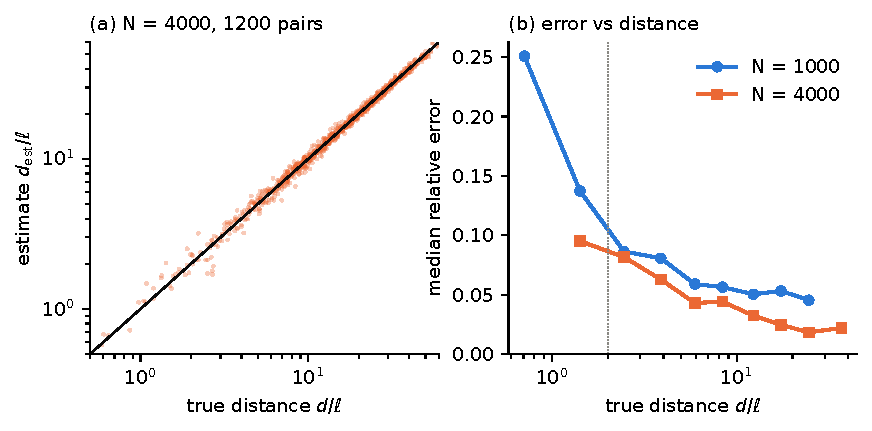
\includegraphics[width=\columnwidth]{fig_distance}
%DIFDELCMD < %%%
\DIFdelendFL \DIFaddbeginFL 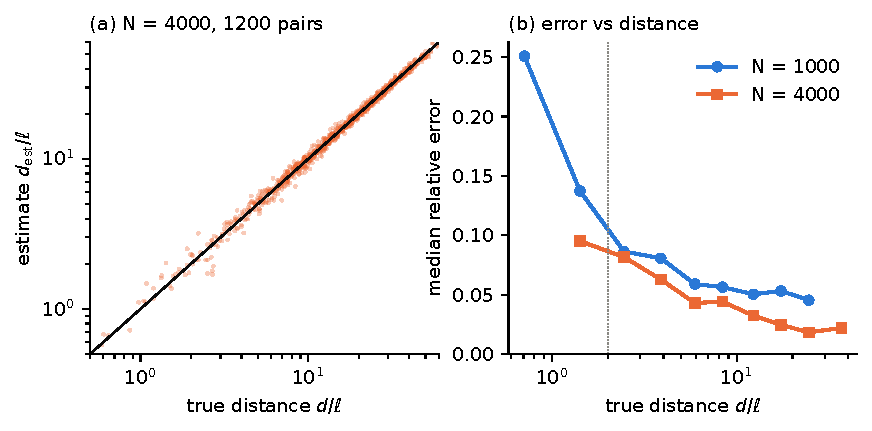
\includegraphics[width=0.8\textwidth]{fig_distance}
\DIFaddendFL \caption{\DIFdelbeginFL \DIFdelFL{Eq.}\DIFdelendFL \DIFaddbeginFL \DIFaddFL{Equation}\DIFaddendFL ~\DIFdelbeginFL \DIFdelFL{\eqref{eq:est} }\DIFdelendFL \DIFaddbeginFL \eref{eq:est} \DIFaddendFL with the deepest $c$ on flat $1+1$ sprinklings, \DIFaddbeginFL \DIFaddFL{computed }\DIFaddendFL from the causal order only. (a) Estimate against true distance, $N=4000$. (b) Median relative error per distance bin; the dotted line marks $2\ell$.}
\label{fig:distance}
\end{figure}

\section{Curvature from depth drift}\label{sec:curv}
In flat spacetime every $c$ in the common past gives the same estimate. In curved spacetime \DIFdelbegin \DIFdel{Eq.~\eqref{eq:rect} }\DIFdelend \DIFaddbegin \DIFadd{equation~}\eref{eq:rect} \DIFaddend no longer holds exactly, and the estimate depends on the depth of $c$. This dependence measures curvature.

\emph{de Sitter volumes.} Two-dimensional de Sitter space in conformal coordinates,
\begin{equation}
\DIFdelbegin \DIFdel{ds}\DIFdelend \DIFaddbegin \rmd \DIFadd{s}\DIFaddend ^2=\DIFdelbegin \DIFdel{\frac{-d\eta^2+dx^2}{(H\eta)^2}}\DIFdelend \DIFaddbegin \DIFadd{\frac{-\rmd\eta^2+\rmd x^2}{(H\eta)^2}}\DIFaddend ,\qquad\eta<0,
\end{equation}
has the light cones of flat space. The tiles $A,B,C,D$ are the same rectangles in $(u,v)=(\eta-x,\eta+x)$, but volumes carry the conformal weight,
\begin{equation}
\DIFdelbegin \DIFdel{dV}\DIFdelend \DIFaddbegin \rmd \DIFadd{V}\DIFaddend =\DIFdelbegin \DIFdel{\frac{d\eta\,dx}{(H\eta)^2}}\DIFdelend \DIFaddbegin \DIFadd{\frac{\rmd\eta\,\rmd x}{(H\eta)^2}}\DIFaddend =\DIFdelbegin \DIFdel{\frac{2\,du\,dv}{H^2(u+v)^2}}\DIFdelend \DIFaddbegin \DIFadd{\frac{2\,\rmd u\,\rmd v}{H^2(u+v)^2}}\DIFaddend .
\end{equation}
\DIFdelbegin \DIFdel{Integrating over }\DIFdelend \DIFaddbegin \DIFadd{When this is integrated over a rectangle }\DIFaddend $[u_1,u_2]\times[v_1,v_2]$, the inner integral gives $1/(u+v_1)-1/(u+v_2)$ and the outer \DIFdelbegin \DIFdel{one }\DIFdelend \DIFaddbegin \DIFadd{integral gives }\DIFaddend a logarithm,
\begin{equation}
V_\square=\frac{2}{H^2}\ln\frac{\eta_L\,\eta_R}{\eta_{\rm bot}\,\eta_{\rm top}},
\label{eq:dsvol}
\end{equation}
with $\eta=(u+v)/2$ evaluated at the left, right, bottom and top corners (all $\eta<0$, so the argument is positive).

\emph{Closed form.} Place $a,b$ on one slice at $(\eta_0,\mp h)$ and $c$ directly below their midpoint at $(\eta_0-T,0)$, and set $H=1$. By symmetry\DIFaddbegin \DIFadd{, }\DIFaddend $V_A=V_B$. \DIFdelbegin \DIFdel{Writing }\DIFdelend \DIFaddbegin \DIFadd{Write }\DIFaddend $\bar\eta=|\eta_0|$ and $q=\bar\eta+T/2$\DIFdelbegin \DIFdel{(}\DIFdelend \DIFaddbegin \DIFadd{, }\DIFaddend so that $|\eta|$ at the corners of $A$ is $q\mp h/2$, $\bar\eta+h$ and $\bar\eta$\DIFdelbegin \DIFdel{), Eq. ~\eqref{eq:dsvol} gives, to }\DIFdelend \DIFaddbegin \DIFadd{. To }\DIFaddend first order in $h$, \DIFaddbegin \DIFadd{equation~}\eref{eq:dsvol} \DIFadd{gives
}\DIFaddend \begin{equation}
V_A=2\ln\frac{(q-\tfrac h2)(\bar\eta+h)}{(q+\tfrac h2)\,\bar\eta}\simeq2h\Big(\frac{1}{\bar\eta}-\frac{1}{q}\Big)=\frac{hT}{\bar\eta\,q},
\end{equation}
and at $h=0$
\begin{equation}
V_C=2\ln\frac{q^2}{(\bar\eta+T)\,\bar\eta}=-2\ln(1-x),\qquad x=\frac{T^2}{4q^2}.
\end{equation}
The true distance is $d\simeq2h/\bar\eta$, so
\begin{equation}
\frac{d^2_{\rm est}}{d^2}=\frac{2V_A^2/V_C}{4h^2/\bar\eta^2}=\frac{x}{-\ln(1-x)}.
\end{equation}
The proper time from $c$ to the midpoint of $a,b$ is $\tau=\ln[(\bar\eta+T)/\bar\eta]$, so that \DIFdelbegin \DIFdel{$T/\bar\eta=e^{\tau}-1$ and $x=[(e^\tau-1)/(e^\tau+1)]^2=\tanh^2(\tau/2)$}\DIFdelend \DIFaddbegin \DIFadd{$T/\bar\eta=\rme^{\tau}-1$ and $x=[(\rme^\tau-1)/(\rme^\tau+1)]^2=\tanh^2(\tau/2)$}\DIFaddend . Restoring $H$,
\begin{equation}
\begin{aligned}
\frac{d^2_{\rm est}}{d^2}&=\frac{\tanh^2(H\tau/2)}{2\ln\cosh(H\tau/2)}=1-\frac{(H\tau)^2}{8}+O(\tau^4)\\
&=1-\frac{R\,\tau^2}{16}+\dots,\qquad R=2H^2,
\end{aligned}
\label{eq:drift}
\end{equation}
\DIFaddbegin \DIFadd{which is }\DIFaddend exact as $d\to0$ at any depth, for $c$ directly below the midpoint of $a$ and $b$. The denominator is $H^2/2$ times the de Sitter volume of an interval of height $\tau$, $V=(4/H^2)\ln\cosh(H\tau/2)$, and the result is independent of $\eta_0$, as required by the de Sitter symmetry. We verified \DIFdelbegin \DIFdel{Eq.~\eqref{eq:drift} }\DIFdelend \DIFaddbegin \DIFadd{equation~}\eref{eq:drift} \DIFaddend against the exact volumes of \DIFdelbegin \DIFdel{Eq.~\eqref{eq:dsvol} }\DIFdelend \DIFaddbegin \DIFadd{equation~}\eref{eq:dsvol} \DIFaddend to $10^{-5}$ for $H\tau=0.1$--$3$. A sideways offset of $c$ changes it little, and a finite $d$ adds an approximately depth-independent shift. We call $1-d^2_{\rm est}/d^2$ the depth drift.

\emph{Other spacetimes.} Every $1+1$ metric is conformally flat, so the leading term should hold locally in any $1+1$ spacetime. We checked this in FRW spacetimes \DIFdelbegin \DIFdel{$ds^2=a(\eta)^2(-d\eta^2+dx^2)$ }\DIFdelend \DIFaddbegin \DIFadd{$\rmd s^2=a(\eta)^2(-\rmd\eta^2+\rmd x^2)$ }\DIFaddend with $a=\eta^p$, where $R=2(\ln a)''/a^2=-2p\,\eta^{-2-2p}$ varies in time and the rectangle volumes have closed forms. For $p=1$, $-2$ and $\tfrac12$ (negative, positive and negative curvature), $16(1-d^2_{\rm est}/d^2)/\tau^2$ tends to $R$ at the location of $a,b$ as $\tau\to0$ (to $1\%$ at $\tau=0.01$), with the correct sign: for $R<0$ the ratio \DIFaddbegin \DIFadd{$d^2_{\rm est}/d^2$ }\DIFaddend exceeds $1$. At finite depth \DIFdelbegin \DIFdel{it }\DIFdelend \DIFaddbegin \DIFadd{the drift }\DIFaddend measures a curvature between the values at $a,b$ and at $c$, with more weight near the top.
\DIFaddbegin 

\DIFaddend The weighting follows from the next order. Write \DIFdelbegin \DIFdel{$a=e^{\sigma(\eta)}$}\DIFdelend \DIFaddbegin \DIFadd{$a=\rme^{\sigma(\eta)}$}\DIFaddend , place $a,b$ at $(\eta_0,\mp h)$\DIFdelbegin \DIFdel{and }\DIFdelend \DIFaddbegin \DIFadd{, and place }\DIFaddend $c$ a coordinate time $T$ straight below. As $h\to0$\DIFaddbegin \DIFadd{, }\DIFaddend the strips have \DIFdelbegin \DIFdel{$V_A=V_B=h\int_0^Te^{2\sigma(\eta_0-s/2)}ds$}\DIFdelend \DIFaddbegin \DIFadd{$V_A=V_B=h\int_0^T\rme^{2\sigma(\eta_0-s/2)}\rmd s$}\DIFaddend , the overlap is \DIFdelbegin \DIFdel{$V_C=\tfrac12\int_0^T\!\!\int_0^Te^{2\sigma(\eta_0-(s+r)/2)}ds\,dr$, and $d=2he^{\sigma(\eta_0)}$. Expanding }\DIFdelend \DIFaddbegin \DIFadd{$V_C=\tfrac12\int_0^T\!\!\int_0^T\rme^{2\sigma(\eta_0-(s+r)/2)}\rmd s\,\rmd r$, and $d=2h\rme^{\sigma(\eta_0)}$. We expand }\DIFaddend $\sigma$ in a Taylor series at $\eta_0$, \DIFdelbegin \DIFdel{integrating }\DIFdelend \DIFaddbegin \DIFadd{integrate }\DIFaddend term by term, and \DIFdelbegin \DIFdel{trading }\DIFdelend \DIFaddbegin \DIFadd{trade }\DIFaddend $T$ for the proper time \DIFdelbegin \DIFdel{$\tau=\int_0^Te^{\sigma(\eta_0-s)}ds$ gives
}\DIFdelend \DIFaddbegin \DIFadd{$\tau=\int_0^T\rme^{\sigma(\eta_0-s)}\rmd s$. This gives
}\DIFaddend \begin{equation}
1-\frac{d^2_{\rm est}}{d^2}=\frac{\tau^2}{16}\Big[R-\frac{\tau}{3}\,\DIFdelbegin \DIFdel{\frac{dR}{d\tau}}\DIFdelend \DIFaddbegin \DIFadd{\frac{\rmd R}{\rmd\tau}}\DIFaddend +O(\tau^2)\Big],
\label{eq:kernel}
\end{equation}
with \DIFdelbegin \DIFdel{$R=2\sigma''e^{-2\sigma}$ }\DIFdelend \DIFaddbegin \DIFadd{$R=2\sigma''\rme^{-2\sigma}$ }\DIFaddend and its derivative along the worldline (toward the future) evaluated at $a,b$. To this order\DIFaddbegin \DIFadd{, }\DIFaddend the drift measures $R$ one third of the way from $a,b$ down to $c$. \DIFdelbegin \DIFdel{Only }\DIFdelend \DIFaddbegin \DIFadd{Equation~}\eref{eq:kernel} \DIFadd{fixes only }\DIFaddend this first moment of the depth weighting\DIFdelbegin \DIFdel{is fixed by Eq. ~\eqref{eq:kernel}; a }\DIFdelend \DIFaddbegin \DIFadd{. A }\DIFaddend triangular weight $2(\tau-s)/\tau^2$ on the depths $s\in[0,\tau]$ is one illustration with this mean depth, not a kernel determined by the expansion\DIFdelbegin \DIFdel{, whose }\DIFdelend \DIFaddbegin \DIFadd{; the }\DIFaddend next order involves $R^2$ and \DIFdelbegin \DIFdel{$d^2R/d\tau^2$ }\DIFdelend \DIFaddbegin \DIFadd{$\rmd^2R/\rmd\tau^2$ }\DIFaddend and is not of the form of a weighted average of $R$. The exact power-law volumes confirm \DIFdelbegin \DIFdel{Eq.~\eqref{eq:kernel}: for }\DIFdelend \DIFaddbegin \DIFadd{equation~}\eref{eq:kernel}\DIFadd{. For }\DIFaddend $p=1$ at $\eta_0=1.5$, $16(1-d^2_{\rm est}/d^2)/\tau^2=-0.3982$, $-0.4073$ \DIFdelbegin \DIFdel{, }\DIFdelend \DIFaddbegin \DIFadd{and }\DIFaddend $-0.4200$ at $\tau=0.02$, $0.05$ \DIFdelbegin \DIFdel{, }\DIFdelend \DIFaddbegin \DIFadd{and }\DIFaddend $0.1$, against $-0.3997$, $-0.4068$ \DIFdelbegin \DIFdel{, }\DIFdelend \DIFaddbegin \DIFadd{and }\DIFaddend $-0.4185$ from its two terms ($R=-0.395$ at $a,b$); the other two values of $p$ agree equally well.

\emph{Test on sprinklings.} We sprinkle de Sitter space ($H=1$, $\rho=10^4$) and, as a control, flat space in the same coordinates\DIFdelbegin \DIFdel{, }\DIFdelend \DIFaddbegin \DIFadd{. We }\DIFaddend insert $a,b$ by hand $\approx14\ell$ apart \DIFdelbegin \DIFdel{, and evaluate Eq.~\eqref{eq:est} }\DIFdelend \DIFaddbegin \DIFadd{and evaluate equation~}\eref{eq:est} \DIFaddend for every sprinkled $c$ in their common past such that the smallest rectangle containing $I(c,a)$ and $I(c,b)$ lies in the region. This cut is stricter than the window of the fit below, which requires only the two intervals to lie in the region. Figure~\ref{fig:drift} shows the mean ratio per depth bin over 400 sprinklings against the continuum value computed for the same elements $c$\DIFdelbegin \DIFdel{, which }\DIFdelend \DIFaddbegin \DIFadd{. The continuum value }\DIFaddend includes the effects of finite $d$ and of sideways offsets\DIFaddbegin \DIFadd{, }\DIFaddend and therefore lies slightly below \DIFdelbegin \DIFdel{Eq.~\eqref{eq:drift}}\DIFdelend \DIFaddbegin \DIFadd{equation~}\eref{eq:drift}\DIFaddend . The flat control remains at $1$\DIFaddbegin \DIFadd{, }\DIFaddend and de Sitter follows the continuum. Neighboring depth bins share elements\DIFdelbegin \DIFdel{: computed }\DIFdelend \DIFaddbegin \DIFadd{. Computed }\DIFaddend from the spread over the 400 sprinklings, the correlation of adjacent bins is $0.80$, $0.81$, $0.90$, $0.94$ \DIFdelbegin \DIFdel{, }\DIFdelend \DIFaddbegin \DIFadd{and }\DIFaddend $0.96$ in de Sitter space (from the shallowest pair \DIFaddbegin \DIFadd{of bins }\DIFaddend to the deepest) and $0.80$--$0.97$ in flat space\DIFdelbegin \DIFdel{, and }\DIFdelend \DIFaddbegin \DIFadd{; }\DIFaddend bins two apart are still correlated at $0.5$--$0.9$. A run of deviations in adjacent bins therefore counts as a single fluctuation, and the points of \DIFdelbegin \DIFdel{Fig.}\DIFdelend \DIFaddbegin \DIFadd{figure}\DIFaddend ~\ref{fig:drift} must not be combined as independent. In the shallowest bin the tile $C$ contains few elements, \DIFdelbegin \DIFdel{the factor $1-e^{-\lambda_C}$ of Eq.~\eqref{eq:est} }\DIFdelend \DIFaddbegin \DIFadd{so the factor $1-\rme^{-\lambda_C}$ of equation~}\eref{eq:est} \DIFaddend is not negligible, and the estimator reads low in both geometries.

\begin{figure}[t]
\centering
\DIFdelbeginFL %DIFDELCMD < 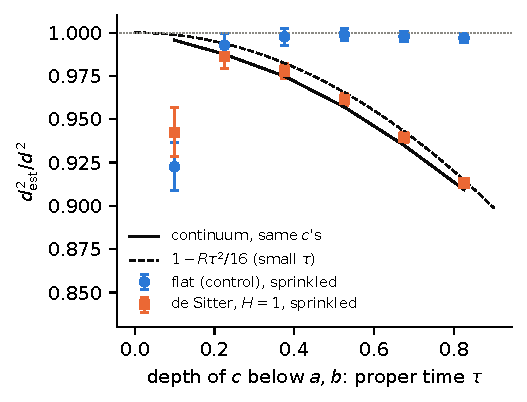
\includegraphics[width=0.85\columnwidth]{fig_drift}
%DIFDELCMD < %%%
\DIFdelendFL \DIFaddbeginFL 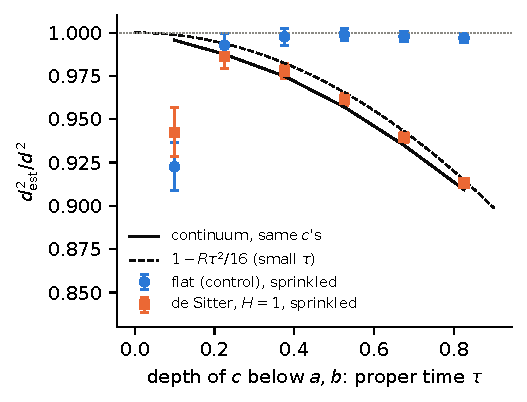
\includegraphics[width=0.6\textwidth]{fig_drift}
\DIFaddendFL \caption{Depth drift of the rectangle estimate: mean over 400 sprinklings ($\rho=10^4$, $H=1$) per bin of the proper time $\tau$ from $c$ to $a,b$, with errors from the spread between sprinklings. The bins are strongly correlated (adjacent bins $0.8$--$0.97$; see text), so the error bars are not independent. Solid: continuum ratio from the exact volumes, averaged over the same elements $c$ (finite $d$ and offsets included). Dashed: small-$\tau$ term of \DIFdelbeginFL \DIFdelFL{Eq.}\DIFdelendFL \DIFaddbeginFL \DIFaddFL{equation}\DIFaddendFL ~\DIFdelbeginFL \DIFdelFL{\eqref{eq:drift}}\DIFdelendFL \DIFaddbeginFL \eref{eq:drift}\DIFaddendFL .}
\label{fig:drift}
\end{figure}

\emph{A curvature estimator.} For one pair $a,b$ we fit $\widehat{d^2}=\alpha+\beta\tau^2$ over the elements $c$ of their common past, with $\tau^2=(N_{I(c,a)}+N_{I(c,b)})/\rho$ from counts, and read \DIFaddbegin \DIFadd{off }\DIFaddend $R=-16\beta/\alpha$. Two choices need care\DIFaddbegin \DIFadd{: the fit window and the way pairs are combined}\DIFaddend .

\emph{Window from the order.} The fit uses every $c$ with $N_C\geq20$, which keeps the factor \DIFdelbegin \DIFdel{$1-e^{-\lambda_C}$ of Eq.~\eqref{eq:est} }\DIFdelend \DIFaddbegin \DIFadd{$1-\rme^{-\lambda_C}$ of equation~}\eref{eq:est} \DIFaddend negligible, down to the deepest $c$ whose intervals $I(c,a)$ and $I(c,b)$ lie in the sprinkled region. Neither limit refers to $H$. The estimator counts only $A$, $B$ and $C$, which lie in $I(c,a)\cup I(c,b)$; the tile $D$ is never counted. In a causally convex region that contains $c$, $a$ and $b$, these intervals lie in the region. On a sprinkling of a causally convex region, for example an interval of the causal set, every $c$ in the common past can therefore be used, \DIFdelbegin \DIFdel{so }\DIFdelend \DIFaddbegin \DIFadd{and }\DIFaddend the window needs no coordinates\DIFdelbegin \DIFdel{; otherwise }\DIFdelend \DIFaddbegin \DIFadd{. Otherwise }\DIFaddend the boundary must first be inferred, which in $1+1$ dimensions is possible from the order~\cite{Cunningham18}. Convexity is an assumption about the sprinkled region: the order decides it only when the causal set is itself defined from the order, as an interval is. Our main tests use a coordinate box, where we decide the condition from the coordinates. We therefore repeated them in a causally convex region, the past of the point $(-0.95,0)$ cut at $\eta=-3$ (convex, although the cut is not defined by the order), \DIFdelbegin \DIFdel{with }\DIFdelend \DIFaddbegin \DIFadd{using }\DIFaddend every $c$ of the common past \DIFdelbegin \DIFdel{used }\DIFdelend (1000 sprinklings each). The results agree with \DIFdelbegin \DIFdel{Table~\ref{tab:rest}: in }\DIFdelend \DIFaddbegin \DIFadd{table~\ref{tab:rest}. In }\DIFaddend de Sitter space the pooled estimate \DIFaddbegin \DIFadd{(defined below) }\DIFaddend is $2.10\pm0.09$ and $2.03\pm0.06$ with inserted pairs\DIFaddbegin \DIFadd{, }\DIFaddend and $2.10\pm0.08$ and $2.04\pm0.06$ with all pairs in the windows \DIFaddbegin \DIFadd{(see below)}\DIFaddend , at $\rho=4000$ and $10^4$ \DIFaddbegin \DIFadd{respectively}\DIFaddend , against continuum values \DIFaddbegin \DIFadd{of }\DIFaddend $2.03$ and $2.04$ (the deeper region changes the target\DIFdelbegin \DIFdel{, }\DIFdelend \DIFaddbegin \DIFadd{; }\DIFaddend see below)\DIFdelbegin \DIFdel{; in flat space }\DIFdelend \DIFaddbegin \DIFadd{. In flat space it is }\DIFaddend $0.01\pm0.02$ and $0.00\pm0.02$ at $\rho=4000$, and $0.00\pm0.01$ and $-0.01\pm0.01$ at $\rho=10^4$.
\DIFaddbegin 

\DIFaddend Because this window reaches $H\tau\approx1$, the $\tau^4$ term of \DIFdelbegin \DIFdel{Eq.~\eqref{eq:drift} contributes, and the }\DIFdelend \DIFaddbegin \DIFadd{equation~}\eref{eq:drift} \DIFadd{contributes. The }\DIFaddend same fit applied to the exact continuum volumes of the same elements gives $R_{\rm fit}^{\rm cont}=2.07$--$2.08$ in the de Sitter box (and $2.03$--$2.04$ in the convex region) instead of $2$. \DIFdelbegin \DIFdel{This}\DIFdelend \DIFaddbegin \DIFadd{The estimator reproduces this value}\DIFaddend , not $2$\DIFdelbegin \DIFdel{, is the value the estimator reproduces; since it }\DIFdelend \DIFaddbegin \DIFadd{. Since the value }\DIFaddend is not known in practice, the difference is a systematic \DIFaddbegin \DIFadd{error }\DIFaddend of the method, of $+2$ to $+4\%$ here, which depends on the size of the region. \DIFdelbegin \DIFdel{Varying }\DIFdelend \DIFaddbegin \DIFadd{We varied }\DIFaddend the lower cut ($N_C\geq5$, $20$, $50$) and the upper cut ($\tau^2$ up to $50\%$, $75\%$ or $100\%$ of its largest value)\DIFdelbegin \DIFdel{changes }\DIFdelend \DIFaddbegin \DIFadd{. These changes move }\DIFaddend the pooled de Sitter result only between $1.91$ and $2.01$ at $\rho=10^4$ (flat: $-0.01$ to $0.00$), within $0.06$--$0.28$ of the continuum value of each rule; the largest offset belongs to the shortest window, which is also the noisiest.

\emph{Pooling.} A single pair gives a noisy estimate (standard deviation $3.5$ at $\rho=4000$ and $2.4$ at $\rho=10^4$ in de Sitter space), and the mean of single-pair values is biased low\DIFdelbegin \DIFdel{: }\DIFdelend \DIFaddbegin \DIFadd{. The reason is that }\DIFaddend the intercept and slope of one least-squares fit have anticorrelated errors, so $E[-16\beta/\alpha]$ is smaller than $-16E[\beta]/E[\alpha]$. Summing the fit coefficients over the pairs before forming the ratio, $R_{\rm est}=-16\sum\beta/\sum\alpha$, removes this ratio bias to first order. Table~\ref{tab:rest} shows the pooled estimator over 1000 sprinklings, with errors from a bootstrap over sprinklings. With inserted pairs it agrees with the continuum value of the same fit\DIFdelbegin \DIFdel{, }\DIFdelend \DIFaddbegin \DIFadd{: }\DIFaddend in flat space within the errors\DIFaddbegin \DIFadd{, }\DIFaddend and in de Sitter space within $0.9\sigma$ and $1.1\sigma$ (offsets \DIFaddbegin \DIFadd{of }\DIFaddend $-0.095\pm0.111$ and $-0.081\pm0.072$ before rounding).

\emph{Sprinkled pairs.} How $a$ and $b$ are chosen among the sprinkled elements matters. Taking the elements nearest to two target points selects elements with an empty neighbo\DIFdelbegin \DIFdel{u}\DIFdelend rhood (the nearest point lies on the boundary of an empty disc), and part of that disc lies at the shallow ends of the strips $A$ and $B$. The counts confirm \DIFdelbegin \DIFdel{it}\DIFdelend \DIFaddbegin \DIFadd{this}\DIFaddend : averaged over the elements $c$ of the window, $N_A-\rho V_A$ is lower by $0.2$--$0.4$ elements than for inserted pairs, at every depth. Since $\lambda_A$ grows with the depth of $c$, a fixed deficit lowers $\widehat{d^2}$ most for shallow $c$\DIFdelbegin \DIFdel{, which }\DIFdelend \DIFaddbegin \DIFadd{. This }\DIFaddend tilts the fitted slope upward and gives \DIFdelbegin \DIFdel{$R$ low }\DIFdelend \DIFaddbegin \DIFadd{a low $R$}\DIFaddend , in flat space as well; the effect shrinks with density. With this selection the estimator reads low in de Sitter space by $0.37\pm0.11$ at $\rho=4000$ and \DIFaddbegin \DIFadd{by }\DIFaddend $0.24\pm0.07$ at $\rho=10^4$ (\DIFdelbegin \DIFdel{Table}\DIFdelend \DIFaddbegin \DIFadd{table}\DIFaddend ~\ref{tab:rest}).
\DIFaddbegin 

\DIFaddend The unbiased use of sprinkled pairs follows from the Mecke formula~\cite{LastPenrose17}: a sum over all pairs of points of a Poisson process, with a weight that depends only on the positions of the pair and not on the rest of the configuration, equals the average over pairs placed by hand at the same positions. The \DIFdelbegin \DIFdel{condition is therefore a }\DIFdelend \DIFaddbegin \DIFadd{requirement is therefore to }\DIFaddend sum over all pairs of a selection that does not depend on the counts used by the estimator, optionally thinned at random with a fixed probability\DIFdelbegin \DIFdel{; the ratio is formed }\DIFdelend \DIFaddbegin \DIFadd{, and to form the ratio }\DIFaddend from the pooled sums. We therefore take every spacelike pair with $a$ in a square window of half-width $0.025$ \DIFaddbegin \DIFadd{($\approx2.5\ell$ at $\rho=10^4$) }\DIFaddend around one target point and $b$ in the window around the other\DIFdelbegin \DIFdel{($\approx2.5\ell$ at $\rho=10^4$), }\DIFdelend \DIFaddbegin \DIFadd{. We }\DIFaddend keep each pair with a fixed probability\DIFaddbegin \DIFadd{, }\DIFaddend chosen so that about $20$ pairs per sprinkling remain, and pool them all. This removes most of the shortfall\DIFdelbegin \DIFdel{: }\DIFdelend \DIFaddbegin \DIFadd{. In de Sitter space }\DIFaddend the pooled estimate is $1.91\pm0.10$ and $2.02\pm0.06$ \DIFdelbegin \DIFdel{in de Sitter space }\DIFdelend against continuum values \DIFaddbegin \DIFadd{of }\DIFaddend $2.08$ ($1.7\sigma$ and $1.1\sigma$ below, against $0.9\sigma$ and $1.1\sigma$ for inserted pairs), and \DIFdelbegin \DIFdel{$0.00\pm0.02$ and $-0.01\pm0.01$ }\DIFdelend in flat space \DIFdelbegin \DIFdel{(Table}\DIFdelend \DIFaddbegin \DIFadd{it is $0.00\pm0.02$ and $-0.01\pm0.01$ (table}\DIFaddend ~\ref{tab:rest}); in the causally convex region it is $2.10\pm0.08$ and $2.04\pm0.06$ against $2.03$ and $2.04$. Drawing a single pair uniformly from the two windows \DIFdelbegin \DIFdel{lies }\DIFdelend \DIFaddbegin \DIFadd{gives results }\DIFaddend in between ($1.80\pm0.11$ and $1.90\pm0.07$): choosing one element out of the $N_W$ in a window weights each configuration by $1/N_W$, which removes about one element from the window. In practice, therefore, the estimator \DIFdelbegin \DIFdel{is to }\DIFdelend \DIFaddbegin \DIFadd{must }\DIFaddend be pooled over all pairs of a position-based selection, not over a single representative chosen per region. A selection by count-defined separation does not satisfy the condition, because it depends on the same counts as the estimator\DIFdelbegin \DIFdel{, and }\DIFdelend \DIFaddbegin \DIFadd{; }\DIFaddend we have not tested it.

\emph{FRW spacetime.} We repeated the test in the $p=1$ FRW spacetime ($\rho=10^4$, 1000 sprinklings), with $a,b$ inserted $14\ell$ apart at $\eta_0=1.5$, \DIFaddbegin \DIFadd{using }\DIFaddend the pooled estimator and the window of the previous paragraphs\DIFdelbegin \DIFdel{, in a causally convex region }\DIFdelend \DIFaddbegin \DIFadd{. The region is causally convex }\DIFaddend (the past of an element at $\eta=1.55$) \DIFaddbegin \DIFadd{and is }\DIFaddend cut at three depths. \DIFdelbegin \DIFdel{With windows reaching }\DIFdelend \DIFaddbegin \DIFadd{The resulting windows reach }\DIFaddend $\tau=0.52$, $0.70$ and $0.84$, over which $R$ ranges from $-0.40$ at $a,b$ to $-1.37$, $-2.79$ and $-6.32$\DIFdelbegin \DIFdel{, the }\DIFdelend \DIFaddbegin \DIFadd{. The }\DIFaddend pooled estimate is $-1.03\pm0.37$, $-0.88\pm0.18$ and $-0.93\pm0.11$, against $-0.70$, $-0.79$ and $-0.90$ for the same fit on the exact volumes of the same elements: the estimator reproduces its continuum target within $1\sigma$. That target is not the leading-order prediction of \DIFdelbegin \DIFdel{Eq.~\eqref{eq:kernel}}\DIFdelend \DIFaddbegin \DIFadd{equation~}\eref{eq:kernel}\DIFaddend , which gives $-0.52$, $-0.55$ and $-0.59$ when fitted in the same way. For the middle window the difference splits about evenly between the higher orders in $\tau$ (the exact volumes with $c$ straight below and $d\to0$ give $-0.67$) and the finite separation of $a$ and $b$ (with $d=14\ell$ the same curve gives $-0.80$). Over a realistic window\DIFdelbegin \DIFdel{Eq.~\eqref{eq:kernel} }\DIFdelend \DIFaddbegin \DIFadd{, equation~}\eref{eq:kernel} \DIFaddend therefore gives the direction of the effect, a curvature measured below the pair, but falls short of its size by $26$--$35\%$ in the three windows\DIFdelbegin \DIFdel{; the }\DIFdelend \DIFaddbegin \DIFadd{. The }\DIFaddend size is set by the exact continuum fit, which the counts reproduce.

\emph{Comparison with other estimators.} The Benincasa--Dowker operator~\cite{BD10}, in its nonlocal two-dimensional form with smearing parameter $\epsilon$, applied to a constant field at the midpoint of the pair, gives $R=-2B_\epsilon[1]$. On the de Sitter and flat sprinklings above, its single-point standard deviation at $\rho=4000$ is $\approx1.2\times10^3$, $160$ and $23$--$30$ for $\epsilon=0.1$, $0.03$ and $0.01$, \DIFdelbegin \DIFdel{and }\DIFdelend \DIFaddbegin \DIFadd{respectively, and it is }\DIFaddend larger at $\rho=10^4$ ($72$--$82$ at $\epsilon=0.01$), as expected at fixed $\epsilon$. Stronger smearing lowers the spread ($2.7$--$4.5$ at $\epsilon=0.003$), but \DIFdelbegin \DIFdel{then the operator }\DIFdelend \DIFaddbegin \DIFadd{the operator then }\DIFaddend needs the past light cone far beyond our sprinkled region, and the truncation dominates its mean ($+0.7$ in flat space, $+4.7$ in de Sitter space)\DIFdelbegin \DIFdel{; a }\DIFdelend \DIFaddbegin \DIFadd{. A }\DIFaddend fair comparison at small $\epsilon$ needs a much larger region, which we have not run. \DIFdelbegin \DIFdel{Its purpose }\DIFdelend \DIFaddbegin \DIFadd{The purpose of this operator }\DIFaddend is the action rather than a pointwise curvature estimate.

The relevant competitor is the ordering fraction of a causal diamond, the leading chain-abundance route~\cite{RSS13}\DIFdelbegin \DIFdel{, compared here as the methods }\DIFdelend \DIFaddbegin \DIFadd{. We compare the two as they }\DIFaddend would be used: one sprinkled region, one estimate. The region is a causal diamond (an interval of the causal set) in de Sitter space, $u,v\in[-3,-0.95]$ ($H=1$; $2.5\times10^3$ elements at $\rho=4000$ \DIFdelbegin \DIFdel{, }\DIFdelend \DIFaddbegin \DIFadd{and }\DIFaddend $6.3\times10^3$ at $\rho=10^4$), sprinkled 400 times. In each sprinkling we take every spacelike pair with $a$ near the top of the diamond ($\eta_a\in[-1.25,-1.05]$, $|x_a|\leq0.1$) and $b$ at $x_b-x_a\in[0.1,0.2]$, $|\eta_b-\eta_a|\leq0.05$ ($9\ell$--$17\ell$ apart at $\rho=10^4$)\DIFdelbegin \DIFdel{, keep each }\DIFdelend \DIFaddbegin \DIFadd{. We keep each pair }\DIFaddend with a fixed probability, the same in every sprinkling, chosen so that $P$ pairs remain on average (a position-based selection in the sense above), and pool the depth drift over them. We compare with $R=2(f-\tfrac12)/(f_{\rm cont}-\tfrac12)$\DIFaddbegin \DIFadd{, obtained }\DIFaddend from the ordering fraction $f$ of the whole diamond \DIFdelbegin \DIFdel{, }\DIFdelend \DIFaddbegin \DIFadd{and }\DIFaddend calibrated on the exact continuum diamond ($f_{\rm cont}=0.5173$). The errors are the spread between sprinklings.
\DIFaddbegin 

\DIFaddend As mean and standard deviation, the ordering fraction gives $2.05\pm0.80$ at $\rho=4000$ and $1.99\pm0.46$ at $\rho=10^4$\DIFdelbegin \DIFdel{; the }\DIFdelend \DIFaddbegin \DIFadd{. The }\DIFaddend pooled drift gives $1.67\pm2.32$ and $1.95\pm1.34$ for $P=100$, against continuum values \DIFdelbegin \DIFdel{$2.10$ of }\DIFdelend \DIFaddbegin \DIFadd{of $2.10$ for }\DIFaddend the same fit: its spread is about three times larger. Pooling more pairs barely helps (standard deviation $2.78$, $2.50$, $2.32$ \DIFdelbegin \DIFdel{, }\DIFdelend \DIFaddbegin \DIFadd{and }\DIFaddend $2.27$ for $P=10$, $30$, $100$ \DIFdelbegin \DIFdel{, }\DIFdelend \DIFaddbegin \DIFadd{and }\DIFaddend $300$ at $\rho=4000$), because pairs in one region share most of their common pasts. For the same reason\DIFaddbegin \DIFadd{, }\DIFaddend the ratio bias is not averaged away within one region: the estimate reads low by $0.43\pm0.12$ and $0.15\pm0.07$. It is the ratio that is biased, not the sums: forming the ratio from $\sum\beta$ and $\sum\alpha$ pooled over all 400 sprinklings gives $1.96\pm0.12$ and $2.04\pm0.07$. Drawing the pairs one at a time instead ($a$ uniformly among the elements near the top, then $b$ uniformly among those at the required offset) gives the same \DIFaddbegin \DIFadd{result }\DIFaddend within the errors in de Sitter space ($1.63$ and $1.92$).
\DIFdelbegin \DIFdel{In a }\DIFdelend \DIFaddbegin 

\DIFadd{As a control we use a }\DIFaddend flat diamond of the same coordinate size, at a lower density\DIFaddbegin \DIFadd{, }\DIFaddend so that it holds the same number of elements as the de Sitter diamond ($2.5\times10^3$ and $6.3\times10^3$)\DIFdelbegin \DIFdel{, }\DIFdelend \DIFaddbegin \DIFadd{. There }\DIFaddend the ordering fraction gives $0.01\pm0.80$ and $0.03\pm0.50$, and the pooled drift \DIFaddbegin \DIFadd{gives }\DIFaddend $-0.16\pm0.89$ and $-0.05\pm0.54$ (low by $0.16\pm0.04$ and $0.05\pm0.03$). The flat control is matched in element count, not in proper depth\DIFdelbegin \DIFdel{: in }\DIFdelend \DIFaddbegin \DIFadd{. In }\DIFaddend the same coordinates the deepest $c$ lies about $1.85$ below the pairs in flat space, against $\ln(3/1.15)\approx0.96$ in de Sitter space, so the range of $\tau^2$ over which the drift is fitted is about four times longer. That alone makes the flat drift less noisy, so the difference between the two geometries in the \DIFdelbegin \DIFdel{factors below }\DIFdelend \DIFaddbegin \DIFadd{precision factors quoted next }\DIFaddend largely reflects this lever arm, not curvature. As a curvature estimator for a given region, the ordering fraction is therefore more precise, by a factor of about three in de Sitter space and slightly in flat space, and less biased. What the depth drift adds is geometric: the curvature appears as the failure of an exact flat-space identity, it is measured along a specific pair and depth rather than over a whole diamond, and \DIFdelbegin \DIFdel{Eq.~\eqref{eq:kernel} }\DIFdelend \DIFaddbegin \DIFadd{equation~}\eref{eq:kernel} \DIFaddend says where. Other counting routes use Ollivier--Ricci curvature~\cite{BBR26}, \DIFaddbegin \DIFadd{with }\DIFaddend which we have not compared.

\begin{table}[t]
\caption{\DIFaddbeginFL \label{tab:rest}\DIFaddendFL Pooled curvature estimator $R_{\rm est}=-16\sum\beta/\sum\alpha$ over 1000 sprinklings ($H=1$; window as in \DIFdelbeginFL \DIFdelFL{Sec.}\DIFdelendFL \DIFaddbeginFL \DIFaddFL{section}\DIFaddendFL ~\ref{sec:curv}: $N_C\geq20$, down to the deepest $c$ with $I(c,a)$ and $I(c,b)$ in the box). Pairs: inserted by hand at two target points; (nearest) the sprinkled elements nearest to them; (windows) all spacelike pairs of sprinkled elements in windows around them, about 20 per sprinkling (see text). Errors: bootstrap over sprinklings. $R_{\rm fit}^{\rm cont}$: the same fit on the exact continuum volumes of the same elements (de Sitter). Last column: standard deviation of single-pair values (de Sitter).}
\DIFdelbeginFL %DIFDELCMD < \label{tab:rest}
%DIFDELCMD < \begin{ruledtabular}
%DIFDELCMD < \begin{tabular}{rlcccc}
%DIFDELCMD < $\rho$ & pairs & flat & de Sitter & $R_{\rm fit}^{\rm cont}$ & single pair\\
%DIFDELCMD < \hline
%DIFDELCMD < 4000 & inserted & $-0.03\pm0.03$ & $1.97\pm0.11$ & $2.07$ & $3.5$\\
%DIFDELCMD <  & nearest & $-0.07\pm0.03$ & $1.70\pm0.11$ & $2.07$ & $3.6$\\
%DIFDELCMD <  & windows & $0.00\pm0.02$ & $1.91\pm0.10$ & $2.08$ & $3.5$\\
%DIFDELCMD < $10^4$ & inserted & $-0.01\pm0.02$ & $1.99\pm0.07$ & $2.08$ & $2.4$\\
%DIFDELCMD <  & nearest & $-0.04\pm0.02$ & $1.84\pm0.07$ & $2.08$ & $2.4$\\
%DIFDELCMD <  & windows & $-0.01\pm0.01$ & $2.02\pm0.06$ & $2.08$ & $2.4$\\
%DIFDELCMD < \end{tabular}
%DIFDELCMD < \end{ruledtabular}
%DIFDELCMD < %%%
\DIFdelendFL \DIFaddbeginFL \begin{indented}
\item[]\begin{tabular}{@{}rlcccc}
\br
$\rho$ & pairs & flat & de Sitter & $R_{\rm fit}^{\rm cont}$ & single pair\\
\mr
4000 & inserted & $-0.03\pm0.03$ & $1.97\pm0.11$ & $2.07$ & $3.5$\\
 & nearest & $-0.07\pm0.03$ & $1.70\pm0.11$ & $2.07$ & $3.6$\\
 & windows & $0.00\pm0.02$ & $1.91\pm0.10$ & $2.08$ & $3.5$\\
$10^4$ & inserted & $-0.01\pm0.02$ & $1.99\pm0.07$ & $2.08$ & $2.4$\\
 & nearest & $-0.04\pm0.02$ & $1.84\pm0.07$ & $2.08$ & $2.4$\\
 & windows & $-0.01\pm0.01$ & $2.02\pm0.06$ & $2.08$ & $2.4$\\
\br
\end{tabular}
\end{indented}
\DIFaddendFL \end{table}

\section{A supporting diagnostic: the embedding test and its blind spot}\label{sec:embed}
\emph{Embedding.} Given the squared intervals $s_{ij}$ between $M$ sampled elements, classical multidimensional scaling (MDS) with a Lorentzian Gram matrix reconstructs coordinates. Clough and Evans applied it to causal sets and proposed its eigenvalue spectrum as a test of dimension and manifoldlikeness~\cite{CloughEvans16,Clough17}. With $s_{ij}=(x_i-x_j)^{\top}\eta\,(x_i-x_j)$, double centering, $G=-\tfrac12JSJ$ with $J=I-\mathbf1\mathbf1^{\top}/M$, gives $G=X\eta X^{\top}$ for the centered coordinates $X$. A $1+1$ Lorentzian set shows one large negative eigenvalue (time), one large positive eigenvalue (space), and \DIFdelbegin \DIFdel{the }\DIFdelend others near zero; the two \DIFaddbegin \DIFadd{corresponding }\DIFaddend eigenvectors give coordinates up to a Lorentz transformation.

We supply MDS with counts only: $s=-2N(I)/\rho$ for related pairs\DIFdelbegin \DIFdel{and Eq.~\eqref{eq:est} }\DIFdelend \DIFaddbegin \DIFadd{, and equation~}\eref{eq:est} \DIFaddend with the deepest $c$ for spacelike pairs. On $M=150$ elements of a flat sprinkling with $N=2000$, positions are recovered to $0.43\pm0.07\,\ell$ across a region $\approx38\ell$ wide\DIFdelbegin \DIFdel{, and the }\DIFdelend \DIFaddbegin \DIFadd{. The }\DIFaddend best affine map from the reconstructed to the true coordinates, $x_{\rm true}\approx Ax_{\rm rec}+b$, is a Lorentz transformation to within $3$--$10\%$, in the sense that the largest entry of $A^{\top}\eta A-\eta$ is $0.03$--$0.10$ in absolute value. The two large eigenvalues are $\approx\mp2.2$\DIFaddbegin \DIFadd{, }\DIFaddend and all others are below $0.1$, in the coordinate units of the sprinkled region (a unit square in $u,v$).

\emph{Statistics and calibration.} As test statistics we use intrinsic numbers only: $r_+$, the ratio of the second to the first positive eigenvalue; the share of the spectrum in one time and one space direction, $(|\lambda_-|+\lambda_+)/\sum_i|\lambda_i|$; and the \emph{stress}, the rms misfit of the squared intervals by the best $1+1$ Minkowski embedding\DIFaddbegin \DIFadd{, }\DIFaddend relative to their rms. The sample consists of the $M=40$ elements with the largest pasts, after removing elements with no common past with the rest. Figure~\ref{fig:detector}(a) shows the calibration on flat universes (random two-dimensional orders)\DIFdelbegin \DIFdel{: stress }\DIFdelend \DIFaddbegin \DIFadd{. Stress }\DIFaddend and $r_+$ settle only for $N\gtrsim100$ (stress $0.16$, $0.10$ \DIFdelbegin \DIFdel{, }\DIFdelend \DIFaddbegin \DIFadd{and }\DIFaddend $0.08$ at $N=100$, $200$ \DIFdelbegin \DIFdel{, }\DIFdelend \DIFaddbegin \DIFadd{and }\DIFaddend $400$), so the test is used only above this size. Curvature raises the stress: for de Sitter diamonds with fixed $N=400$ it stays in the flat band up to $H\tau\approx1$ and reaches $0.25$ at $H\tau=4$ [\DIFdelbegin \DIFdel{Fig.}\DIFdelend \DIFaddbegin \DIFadd{figure}\DIFaddend ~\ref{fig:detector}(c)]. The stress thus tests whether the order is a \emph{flat} sheet, \DIFdelbegin \DIFdel{while Sec.}\DIFdelend \DIFaddbegin \DIFadd{whereas section}\DIFaddend ~\ref{sec:curv} measures its curvature.

\emph{Blind spot.} Applied to Monte Carlo samples of the \DIFdelbegin \DIFdel{$e^{-\beta S}$ }\DIFdelend \DIFaddbegin \DIFadd{$\rme^{-\beta S}$ }\DIFaddend model at $N=400$ (\DIFdelbegin \DIFdel{Sec.}\DIFdelend \DIFaddbegin \DIFadd{section}\DIFaddend ~\ref{sec:phases}), this test passes every continuum-like state at that size (\DIFaddbegin \DIFadd{but }\DIFaddend not at $N=800$; \DIFdelbegin \DIFdel{Sec.}\DIFdelend \DIFaddbegin \DIFadd{see section}\DIFaddend ~\ref{sec:phases}) and fails orders with 4 and 7 layers\DIFdelbegin \DIFdel{, but it does not}\DIFdelend \DIFaddbegin \DIFadd{. It does not, however, }\DIFaddend reliably flag orders with about 10 layers: at $M=40$ one of seven \DIFaddbegin \DIFadd{such orders }\DIFaddend lies in the flat band and two more \DIFaddbegin \DIFadd{lie }\DIFaddend just above it, and at $M=80$ two others have stress $0.03$, lower than flat orders. Two effects are responsible. \DIFdelbegin \DIFdel{The }\DIFdelend \DIFaddbegin \DIFadd{First, the }\DIFaddend sample contains only the top one or two layers. \DIFdelbegin \DIFdel{And }\DIFdelend \DIFaddbegin \DIFadd{Second, }\DIFaddend in a layered order most sampled pairs have zero squared interval: linked pairs have $N(I)=0$, and spacelike pairs often have an empty strip, $N_A=0$ or $N_B=0$. MDS fits an all-zero matrix perfectly\DIFdelbegin \DIFdel{; }\DIFdelend \DIFaddbegin \DIFadd{, and }\DIFaddend a bilayer produces exactly that \DIFaddbegin \DIFadd{matrix}\DIFaddend .

\emph{Null-pair fraction.} We add the fraction $z$ of sampled pairs with zero squared interval, taken as the larger of its values on the top sample and on a sample spread evenly in height (\DIFaddbegin \DIFadd{the }\DIFaddend longest chain below the element) over the upper $70\%$ of the order. On sprinklings\DIFaddbegin \DIFadd{, }\DIFaddend $z$ decreases with $N$ (median $0.18$, $0.12$ \DIFdelbegin \DIFdel{, }\DIFdelend \DIFaddbegin \DIFadd{and }\DIFaddend $0.09$ at $N=100$, $200$ \DIFdelbegin \DIFdel{, }\DIFdelend \DIFaddbegin \DIFadd{and }\DIFaddend $400$) and does not respond to curvature: de Sitter diamonds at $H\tau=4$ give $0.08$--$0.11$. Layered orders give $0.4$--$1$ [\DIFdelbegin \DIFdel{Fig.}\DIFdelend \DIFaddbegin \DIFadd{figure}\DIFaddend ~\ref{fig:detector}(b)]. We flag an order as layered when $z$ exceeds $1.5$ times the flat median at the same $N$. Orders with only 2--3 layers cannot be processed (too few elements share a common past), and the rule counts them as flagged.

\emph{What $z$ adds.} Layered orders are also detected by simpler statistics: the height (number of layers), the ordering fraction and the Myrheim--Meyer dimension~\cite{Myrheim78,Meyer88}, interval abundances~\cite{GlaserSurya13}, and graph observables~\cite{EMLW26}\DIFdelbegin \DIFdel{; in the $e^{-\beta S}$ literature}\DIFdelend \DIFaddbegin \DIFadd{. In the $\rme^{-\beta S}$ literature, }\DIFaddend the phases are characterized by the action, the ordering fraction, the height and interval abundances~\cite{Surya12,GOS18,GlaserSurya16,Glaser18,Glaser23}. On our states the fixed-size ordering fraction separates the same groups as $z$ (\DIFdelbegin \DIFdel{Appendix~}\DIFdelend \ref{app:prop}). The null-pair fraction does not detect anything \DIFdelbegin \DIFdel{these }\DIFdelend \DIFaddbegin \DIFadd{that these statistics }\DIFaddend miss. Its role is to make the embedding test usable on its own: without \DIFdelbegin \DIFdel{it }\DIFdelend \DIFaddbegin \DIFadd{$z$ }\DIFaddend the test passes some 10-layer orders, so a user who relied on the embedding spectrum alone would accept them. With $z$ the test needs no second statistic, and it uses only quantities \DIFaddbegin \DIFadd{that }\DIFaddend the embedding already computes.

\DIFdelbegin %DIFDELCMD < \begin{figure*}[t]
%DIFDELCMD < %%%
\DIFdelendFL \DIFaddbeginFL \begin{figure}[t]
\DIFaddendFL \centering
\DIFdelbeginFL %DIFDELCMD < 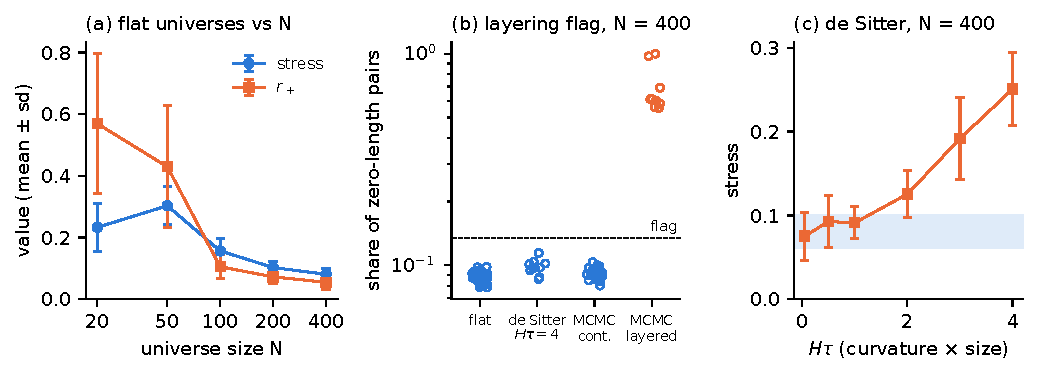
\includegraphics[width=0.9\textwidth]{fig_detector}
%DIFDELCMD < %%%
\DIFdelendFL \DIFaddbeginFL 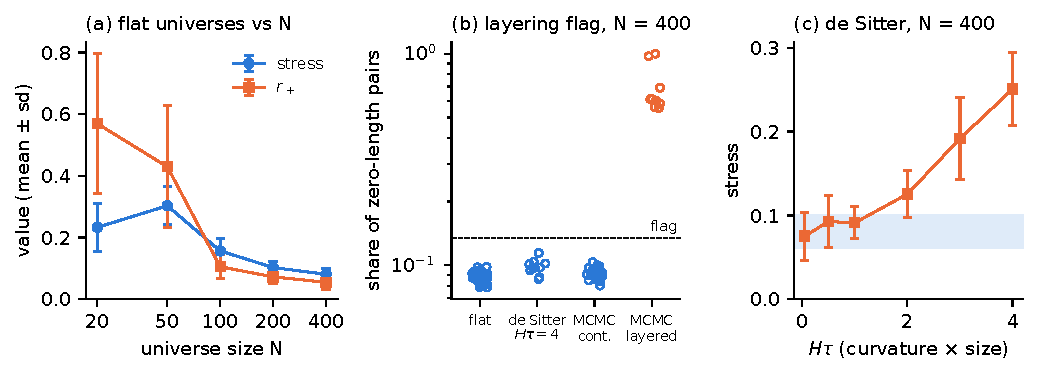
\includegraphics[width=\textwidth]{fig_detector}
\DIFaddendFL \caption{Calibration of the embedding test. (a) Flat universes (random two-dimensional orders, 10 per size, $M=40$): stress and $r_+$ against the number of elements $N$. (b) Null-pair fraction $z$ at $N=400$ ($M=80$) for flat orders, de Sitter diamonds at $H\tau=4$, and final states of \DIFdelbeginFL \DIFdelFL{$e^{-\beta S}$ }\DIFdelendFL \DIFaddbeginFL \DIFaddFL{$\rme^{-\beta S}$ }\DIFaddendFL Monte Carlo chains (continuum-like, 30--39 layers; layered, 4--11 layers). Dashed: the flag threshold, $1.5$ times the flat median. The 13 states with 2--3 layers are not shown. (c) Stress of de Sitter diamonds at fixed $N=400$ (8 per height) against $H\tau$; shaded: the flat band ($\pm1$ standard deviation).}
\label{fig:detector}
\DIFdelbeginFL %DIFDELCMD < \end{figure*}
%DIFDELCMD < %%%
\DIFdelend \DIFaddbegin \end{figure}
\DIFaddend 

\section{Applications}\label{sec:phases}
\emph{Sequential growth.} In transitive percolation, the simplest classical sequential growth model~\cite{RideoutSorkin00}, elements are born one at a time\DIFdelbegin \DIFdel{and }\DIFdelend \DIFaddbegin \DIFadd{, }\DIFaddend each newborn element chooses each existing element as an ancestor with probability $p$, and the order is the transitive closure. As a sanity check of the diagnostics\DIFaddbegin \DIFadd{, }\DIFaddend we grew universes of $N=100$ and $200$ elements with $p=0.05$, and with the non-covariant variant $p_n=3/n$. Neither produces a $1+1$ spacetime\DIFdelbegin \DIFdel{: the }\DIFdelend \DIFaddbegin \DIFadd{. The }\DIFaddend ordering-fraction dimension drifts with scale, and the embedding test fails on every statistic\DIFdelbegin \DIFdel{(}\DIFdelend \DIFaddbegin \DIFadd{: the }\DIFaddend share of the spectrum in one time and one space direction \DIFaddbegin \DIFadd{is }\DIFaddend $\approx0.33$\DIFaddbegin \DIFadd{, }\DIFaddend against $0.65$ for flat orders at $N=100$\DIFdelbegin \DIFdel{; stress }\DIFdelend \DIFaddbegin \DIFadd{, and the stress is }\DIFaddend $0.64$--$0.78$\DIFaddbegin \DIFadd{, }\DIFaddend against $0.10$--$0.12$ at $N=200$\DIFdelbegin \DIFdel{). Their }\DIFdelend \DIFaddbegin \DIFadd{. It is not their }\DIFaddend null-pair \DIFdelbegin \DIFdel{fraction is not what flags them; grown }\DIFdelend \DIFaddbegin \DIFadd{fraction that flags them. Grown }\DIFaddend universes with $N=1500$ also fail the propagator target (\DIFdelbegin \DIFdel{Appendix~}\DIFdelend \ref{app:prop}). Covariant approaches to cosmology in growth models are discussed in\DIFdelbegin \DIFdel{Refs.}\DIFdelend ~\cite{MORS01,AhmedRideout10}.

\emph{The two phases of the \DIFdelbegin \DIFdel{$e^{-\beta S}$ }\DIFdelend \DIFaddbegin \DIFadd{$\rme^{-\beta S}$ }\DIFaddend model.} Weighting two-dimensional orders by \DIFdelbegin \DIFdel{$e^{-\beta S}$}\DIFdelend \DIFaddbegin \DIFadd{$\rme^{-\beta S}$}\DIFaddend , with $S$ the Benincasa--Dowker action, gives a first-order transition between a continuum-like and a layered phase~\cite{BHS08,Surya12,GOS18}. We sampled \DIFdelbegin \DIFdel{it }\DIFdelend \DIFaddbegin \DIFadd{the model }\DIFaddend with Metropolis swap moves at nonlocality parameter $\epsilon=0.21$\DIFdelbegin \DIFdel{(an $O(N^2)$ update }\DIFdelend \DIFaddbegin \DIFadd{. Each update costs $O(N^2)$}\DIFaddend , since a swap changes two rows and columns of the causal matrix\DIFdelbegin \DIFdel{)}\DIFdelend . Table~\ref{tab:phases} shows the diagnostics at $N=200$. The states at $\beta\geq0.6$ are metastable intermediates; the ground state at large $\beta$ is a bilayer~\cite{CunninghamSurya19}.

\begin{table}[t]
\caption{\DIFaddbeginFL \label{tab:phases}\DIFaddendFL Embedding diagnostics on \DIFdelbeginFL \DIFdelFL{$e^{-\beta S}$ }\DIFdelendFL \DIFaddbeginFL \DIFaddFL{$\rme^{-\beta S}$ }\DIFaddendFL states at $N=200$ ($\epsilon=0.21$). $f$: ordering fraction; $L$: number of layers. The last column gives the range of the null-pair fraction $z$ on fresh chains, for $\beta\le0.3$ (second row) and \DIFaddbeginFL \DIFaddFL{for }\DIFaddendFL $\beta\ge0.6$ with 8--13 layers (third row).}
\DIFdelbeginFL %DIFDELCMD < \label{tab:phases}
%DIFDELCMD < \begin{ruledtabular}
%DIFDELCMD < \begin{tabular}{lccccc}
%DIFDELCMD < $N=200$ & $f$ & $L$ & $r_+$ & stress & $z$\\
%DIFDELCMD < \hline
%DIFDELCMD < random orders & 0.50 & 24 & 0.07 & 0.10 & 0.10--0.15\\
%DIFDELCMD < $\beta=0.05$ & 0.51 & 24 & 0.10 & 0.11 & 0.12--0.13\\
%DIFDELCMD < $\beta=0.6$ & 0.59 & 9 & 0.39 & 0.28 & 0.39--0.48\\
%DIFDELCMD < \end{tabular}
%DIFDELCMD < \end{ruledtabular}
%DIFDELCMD < %%%
\DIFdelendFL \DIFaddbeginFL \begin{indented}
\item[]\begin{tabular}{@{}lccccc}
\br
$N=200$ & $f$ & $L$ & $r_+$ & stress & $z$\\
\mr
random orders & 0.50 & 24 & 0.07 & 0.10 & 0.10--0.15\\
$\beta=0.05$ & 0.51 & 24 & 0.10 & 0.11 & 0.12--0.13\\
$\beta=0.6$ & 0.59 & 9 & 0.39 & 0.28 & 0.39--0.48\\
\br
\end{tabular}
\end{indented}
\DIFaddendFL \end{table}

The states below are test configurations, representative of the two phases, not equilibrium samples (see the end of this section). We applied the flag to 44 final states of $N=400$ chains run from random and from layered initial orders at $0.01\leq\beta\leq0.7$. All 22 continuum-like states (30--39 layers) pass\DIFdelbegin \DIFdel{; all }\DIFdelend \DIFaddbegin \DIFadd{. All }\DIFaddend 9 states with 4--11 layers are flagged ($z=0.55$--$1.0$\DIFaddbegin \DIFadd{, }\DIFaddend against a threshold of $0.13$)\DIFdelbegin \DIFdel{; the }\DIFdelend \DIFaddbegin \DIFadd{. The }\DIFaddend 13 states with 2--3 layers cannot be processed and are counted as flagged. The fixed-$n$ ordering fraction (\DIFdelbegin \DIFdel{Appendix~}\DIFdelend \ref{app:prop}) separates the same groups; the propagator statistic misses one 4-layer state.
\DIFaddbegin 

\DIFaddend Because the flag was designed after these states had been seen, we tested it on held-out samples. On fresh $N=200$ chains, 12 of 12 continuum-like states pass and 18 of 18 layered states ($\beta=0.6$--$1.5$) are flagged. At $N=800$ \DIFdelbegin \DIFdel{, with }\DIFdelend \DIFaddbegin \DIFadd{we used }\DIFaddend $M=80$ (as for $z$ at $N=400$) and \DIFdelbegin \DIFdel{the }\DIFdelend \DIFaddbegin \DIFadd{a }\DIFaddend threshold fixed in advance from flat orders\DIFdelbegin \DIFdel{(}\DIFdelend \DIFaddbegin \DIFadd{: }\DIFaddend $z>0.120$, $1.5$ times the median $z=0.080$ of 50 flat orders\DIFdelbegin \DIFdel{; none }\DIFdelend \DIFaddbegin \DIFadd{. None }\DIFaddend of 50 fresh flat orders and 20 de Sitter diamonds is flagged\DIFdelbegin \DIFdel{), we }\DIFdelend \DIFaddbegin \DIFadd{. We }\DIFaddend ran 28 chains ($\beta\in\{0.01,0.05,0.1,0.2,0.3,0.45,0.7\}$, 4 seeds each, random initial orders, 2000 sweeps), with the classes also fixed in advance\DIFdelbegin \DIFdel{(}\DIFdelend \DIFaddbegin \DIFadd{: }\DIFaddend at least 20 layers\DIFdelbegin \DIFdel{: }\DIFdelend \DIFaddbegin \DIFadd{, }\DIFaddend continuum-like; 4--19 layers\DIFdelbegin \DIFdel{: layered). On this }\DIFdelend \DIFaddbegin \DIFadd{, layered. This gives a }\DIFaddend small held-out sample \DIFdelbegin \DIFdel{(}\DIFdelend \DIFaddbegin \DIFadd{of }\DIFaddend 8 layered and 20 continuum-like states\DIFdelbegin \DIFdel{), all }\DIFdelend \DIFaddbegin \DIFadd{. All }\DIFaddend 8 layered states (14--19 layers) are flagged ($z=0.38$--$0.57$)\DIFdelbegin \DIFdel{; only }\DIFdelend \DIFaddbegin \DIFadd{. Only }\DIFaddend one of them, with stress $0.072$, lies in the flat band\DIFdelbegin \DIFdel{, }\DIFdelend \DIFaddbegin \DIFadd{; this is }\DIFaddend the blind spot that $z$ is meant to close, and the embedding spectrum alone would have passed it. Of the 20 continuum-like states (27--56 layers), 19 are not flagged ($z\leq0.107$). The exception has 27 layers at $\beta=0.3$ and is flagged with $z=0.123$, just above the threshold\DIFdelbegin \DIFdel{; its }\DIFdelend \DIFaddbegin \DIFadd{. Its }\DIFaddend acceptance rate ($5\%$, against $53$--$54\%$ for the other three chains at $\beta=0.3$, which reached 43--50 layers) suggests that it is partly layered, but by the classes fixed in advance it is a false positive. For context only: random two-dimensional orders of $800$ elements have $52$ layers on average (standard deviation $2.5$), so this state has about half the flat height, whereas the continuum-like states at $N=400$ had $30$--$39$ layers against a flat mean of $36$. Three of the 19 unflagged states have a stress slightly above the flat band at $N=800$ ($0.086$--$0.110$, against \DIFaddbegin \DIFadd{the }\DIFaddend flat mean plus two standard deviations, $0.081$), as does the flagged one ($0.134$)\DIFdelbegin \DIFdel{, so at this size}\DIFdelend \DIFaddbegin \DIFadd{. At this size, therefore, }\DIFaddend the stress alone would also reject some continuum-like states.
\DIFaddbegin 

\DIFaddend The $N=400$ states are test inputs, not equilibrium samples: chains started from layered orders accept $\leq0.1\%$ of the moves. They bracket the transition only loosely: chains from layered starts become continuum-like at $\beta\leq0.05$, and chains from random starts become layered at $\beta\geq0.45$. The bracket $0.05<\beta_c(400)<0.45$ is compatible with the finite-size scaling $\beta_c\approx1.66/(\epsilon^2N)=0.094$ of\DIFdelbegin \DIFdel{Ref.~\mbox{%DIFAUXCMD
\cite{GOS18}}\hskip0pt%DIFAUXCMD
; }\DIFdelend \DIFaddbegin \DIFadd{~\mbox{%DIFAUXCMD
\cite{GOS18}}\hskip0pt%DIFAUXCMD
, but }\DIFaddend it is too loose to test it.

\section{Discussion}\label{sec:disc}
\emph{What is new.} The overlap regions are those of\DIFdelbegin \DIFdel{Ref.}\DIFdelend ~\cite{BK24}, the embedding test is that of\DIFdelbegin \DIFdel{Ref.}\DIFdelend ~\cite{CloughEvans16}, the null-pair fraction is related to\DIFdelbegin \DIFdel{Ref.}\DIFdelend ~\cite{GlaserSurya13}, and the Laguerre identity is classical combinatorics. To our knowledge\DIFaddbegin \DIFadd{, }\DIFaddend the following are new: the rectangle identity for general $c$, \DIFdelbegin \DIFdel{Eq.~\eqref{eq:rect}}\DIFdelend \DIFaddbegin \DIFadd{equation~}\eref{eq:rect}\DIFaddend , with the bias-corrected estimator and its comparison with existing constructions, including a counting version of the Hu--Meyer--Meyer construction; the depth drift, its closed form in de Sitter space, \DIFdelbegin \DIFdel{Eq.~\eqref{eq:drift}}\DIFdelend \DIFaddbegin \DIFadd{equation~}\eref{eq:drift}\DIFaddend , and its leading form in FRW spacetimes, \DIFdelbegin \DIFdel{Eq.~\eqref{eq:kernel}}\DIFdelend \DIFaddbegin \DIFadd{equation~}\eref{eq:kernel}\DIFaddend , with the curvature estimator built on it; the application of the Laguerre identity to Johnston's propagator, \DIFdelbegin \DIFdel{Eq.~\eqref{eq:lag}}\DIFdelend \DIFaddbegin \DIFadd{equation~}\eref{eq:lag}\DIFaddend ; and the calibration of the embedding test against size, curvature and layering. Our literature search (October 2026) covered the \DIFdelbegin \DIFdel{citing papers of Refs.~\mbox{%DIFAUXCMD
\cite{BK24,CloughEvans16,Johnston08,Johnston09}}\hskip0pt%DIFAUXCMD
; the }\DIFdelend \DIFaddbegin \DIFadd{papers citing~\mbox{%DIFAUXCMD
\cite{BK24,CloughEvans16,Johnston08,Johnston09}}\hskip0pt%DIFAUXCMD
. The }\DIFaddend rectangle identity is elementary enough that it may appear in passing in work we did not reach.

\emph{What the curvature result is.} Since the ordering fraction of a region is the more precise estimate of its curvature, the curvature result of this paper is analytic and conceptual: an exact flat-space identity whose depth-dependent failure has a closed form, \DIFdelbegin \DIFdel{Eq.~\eqref{eq:drift}}\DIFdelend \DIFaddbegin \DIFadd{equation~}\eref{eq:drift}\DIFaddend , and a leading-order meaning, \DIFdelbegin \DIFdel{Eq.~\eqref{eq:kernel}}\DIFdelend \DIFaddbegin \DIFadd{equation~}\eref{eq:kernel}\DIFaddend . Whether the locality of the depth drift, a curvature along one pair and one depth, makes it the better estimator where curvature varies across a region is untested. A methodological point is of more general use\DIFdelbegin \DIFdel{: estimators }\DIFdelend \DIFaddbegin \DIFadd{. Estimators }\DIFaddend evaluated on sprinkled elements chosen as the nearest to given points, or one per window, inherit a Palm-type selection bias, because the choice depends on the neighbo\DIFdelbegin \DIFdel{u}\DIFdelend rhood that the estimator counts\DIFdelbegin \DIFdel{; summing }\DIFdelend \DIFaddbegin \DIFadd{. Summing }\DIFaddend over all elements or pairs of a position-based selection, as the Mecke formula requires, removes it.

\emph{Limitations.} The exact results are specific to $1+1$ dimensions\DIFdelbegin \DIFdel{; the }\DIFdelend \DIFaddbegin \DIFadd{. The }\DIFaddend rectangle identity has no direct analogue in higher dimensions, where the overlap of two intervals is not an interval. The distance estimator is the most accurate only below about $10\ell$; at larger separations the counting version of the Hu--Meyer--Meyer construction is better. The curvature estimator must be pooled over all pairs of a position-based selection and over many independent regions; within one region the ratio stays biased (\DIFaddbegin \DIFadd{see }\DIFaddend below). Single pairs are dominated by noise and their ratio is biased, and selecting the elements nearest to given points, or one element per window, biases it low. \DIFdelbegin \DIFdel{Its target }\DIFdelend \DIFaddbegin \DIFadd{The target of the estimator }\DIFaddend is the same fit on the continuum volumes, not $R$ itself. Because the window reaches $H\tau\approx1$, the $\tau^4$ term of \DIFdelbegin \DIFdel{Eq.~\eqref{eq:drift} }\DIFdelend \DIFaddbegin \DIFadd{equation~}\eref{eq:drift} \DIFaddend makes this target $2.07$--$2.08$ instead of $2$ in our de Sitter box\DIFaddbegin \DIFadd{, }\DIFaddend and $2.03$--$2.04$ in the convex region\DIFdelbegin \DIFdel{: a systematic of }\DIFdelend \DIFaddbegin \DIFadd{. This is a systematic error of the method, of }\DIFaddend $+2$ to $+4\%$\DIFdelbegin \DIFdel{of the method}\DIFdelend , which depends on the size of the region and is not known in practice; capping the window lowers it at the cost of noise (\DIFdelbegin \DIFdel{Sec.}\DIFdelend \DIFaddbegin \DIFadd{section}\DIFaddend ~\ref{sec:curv}). In FRW spacetime the leading-order prediction of \DIFdelbegin \DIFdel{Eq.~\eqref{eq:kernel} }\DIFdelend \DIFaddbegin \DIFadd{equation~}\eref{eq:kernel} \DIFaddend falls short of this target by $26$--$35\%$ over realistic windows. Within one region the pairs share elements, so pooling more than a few tens of them gains little\DIFaddbegin \DIFadd{, }\DIFaddend and the estimate retains a low ratio bias of $0.05$--$0.43$ at the densities used\DIFdelbegin \DIFdel{; for }\DIFdelend \DIFaddbegin \DIFadd{. For }\DIFaddend the curvature of a given region the ordering fraction is more precise, by a factor of about three in de Sitter space, and less biased. The estimator was tested on de Sitter space and \DIFaddbegin \DIFadd{on }\DIFaddend one FRW spacetime. The embedding thresholds are empirical and must be recalibrated at each $N$\DIFdelbegin \DIFdel{; on }\DIFdelend \DIFaddbegin \DIFadd{. On }\DIFaddend a small held-out sample at $N=800$ (8 layered and 20 continuum-like states)\DIFaddbegin \DIFadd{, }\DIFaddend the layered flag caught every layered state but also one of the 20 continuum-like states, just above its threshold\DIFdelbegin \DIFdel{; the }\DIFdelend \DIFaddbegin \DIFadd{. The }\DIFaddend stress put that state ($0.134$) and 3 of the 19 unflagged ones above the flat band, so at this size the full embedding test (spectrum, stress and $z$) rejects 4 of the 20 continuum-like states\DIFdelbegin \DIFdel{; the $e^{-\beta S}$ }\DIFdelend \DIFaddbegin \DIFadd{. The $\rme^{-\beta S}$ }\DIFaddend states used are test inputs, not equilibrium samples. The Laguerre target is exact only for two-dimensional orders, and as a manifoldlikeness diagnostic it is not stronger than the ordering fraction.

\emph{Outlook.} Since the Hu--Meyer--Meyer construction is the more accurate one at large separations, a depth drift built on it may be less noisy there; a combined distance estimator would switch between the two near $10\ell$. A fixed-$n$ propagator target in $3+1$ dimensions would not be exact\DIFdelbegin \DIFdel{: }\DIFdelend \DIFaddbegin \DIFadd{. }\DIFaddend Johnston's $3+1$ particle hops along links only~\cite{Johnston08}, so a path requires every skipped sub-interval to be empty, and $E[K\,|\,n]$ becomes a sum of $(k-1)$-point integrals with factors $(1-W/V)^{n-k+1}$. Its first term can be evaluated at large $n$: the expected number of two-hop link paths tends to $3\pi$\DIFdelbegin \DIFdel{, which }\DIFdelend \DIFaddbegin \DIFadd{. This }\DIFaddend is what Johnston's amplitudes require to reproduce the short-distance limit $m^2/8\pi$ of the continuum mass term~\cite{Johnston08}, so \DIFdelbegin \DIFdel{this }\DIFdelend \DIFaddbegin \DIFadd{it }\DIFaddend is a consistency check rather than a new result; a Monte Carlo evaluation approaches it as $3\pi(1-1.6/\sqrt n)$ at fixed $n$. A $3+1$ target would therefore be a computed table rather than a formula.

\section*{Data availability \DIFaddbegin \DIFadd{statement}\DIFaddend }
\DIFaddbegin {\sloppy
\DIFaddend The code that produces every number and figure in this paper, and the research notebook in which the work was carried out, are openly available at \url{https://github.com/presindev/causet-counting}, and the version used for this paper is archived at doi:\pending{Zenodo DOI}. Figures are produced by \texttt{sims/fig\_part1.py}; the baseline comparison by \texttt{sims/r31\_rect\_baseline.py} and, with the Hu--Meyer--Meyer construction and the ablations, \DIFaddbegin \DIFadd{by }\DIFaddend \texttt{sims/r36\_rect\_ablation\_hmm.py}; the curvature estimator (window, pooled form, sprinkled pairs, Benincasa--Dowker and chain-abundance comparison, bin correlations) by \texttt{sims/r37\_curvature\_referee.py}; the sprinkled-pair selections, the causally convex region, the FRW test with the pooled estimator and the first comparison with the ordering fraction in one region by \texttt{sims/r40\_curvature\_round2.py}; the one-region comparison with a position-based selection and the flat control at matched element count by \texttt{sims/r41\_curvature\_round3.py}; \DIFdelbegin \DIFdel{Eq.~\eqref{eq:kernel} }\DIFdelend \DIFaddbegin \DIFadd{equation~}\eref{eq:kernel} \DIFaddend by \texttt{sims/r38\_drift\_kernel.py}; the null-pair fraction by \texttt{sims/r8\_detector\_spread.py}; the curvature fit and the FRW check by \texttt{sims/r9\_drift\_fit\_frw.py}; the \DIFdelbegin \DIFdel{$e^{-\beta S}$ }\DIFdelend \DIFaddbegin \DIFadd{$\rme^{-\beta S}$ }\DIFaddend states by \texttt{sims/n400\_crystal.py}; the propagator statistics by \texttt{sims/b\_johnston\_n400.py} and \texttt{sims/r32\_laguerre\_vs\_fraction.py}; \DIFaddbegin \DIFadd{and }\DIFaddend the $N=800$ test by \texttt{sims/r27\_n800\_detector.py}, \DIFdelbegin \DIFdel{and }\DIFdelend \DIFaddbegin \DIFadd{with }\DIFaddend the heights of random orders quoted with it by \texttt{sims/r42\_flat\_height.py}.\DIFaddbegin \par}
\DIFaddend 

\DIFdelbegin %DIFDELCMD < \begin{acknowledgments}
%DIFDELCMD < %%%
\DIFdelend \DIFaddbegin \ack
\DIFaddend This work was funded by SapereIA. Simulations were run on the Nyx cluster of the Institute of Cosmos Sciences of the University of Barcelona (ICCUB). An AI system (Claude Opus~5.5, Anthropic) was used for literature search, derivations, code and drafting, under the author's direction and checks; the procedure is described in\DIFdelbegin \DIFdel{Ref.}\DIFdelend ~\cite{MethodNote}. The author takes full responsibility for the content.
\DIFdelbegin %DIFDELCMD < \end{acknowledgments}
%DIFDELCMD < %%%
\DIFdelend 

\appendix
\section{A density-free target for Johnston's propagator}\label{app:prop}
This appendix records a combinatorial identity for Johnston's propagator. As a diagnostic of manifoldlikeness it is not stronger than the ordering fraction (\DIFaddbegin \DIFadd{see the }\DIFaddend end of this appendix); its use is as an exact, density-free check of implementations of the chain sum.

\emph{The propagator.} In Johnston's model a particle hops along the order with amplitude $a$ per hop and $b$ per intermediate stop~\cite{Johnston08}. With $C$ the causal matrix ($C_{xy}=1$ if $x\prec y$) and $\Phi=aC$,
\begin{equation}
K=\Phi+b\,\Phi^2+b^2\Phi^3+\dots=\Phi\,(I-b\Phi)^{-1},
\end{equation}
with $a=\tfrac12$ and $b=-m^2/\rho$ in $1+1$ dimensions. $K(x,y)$ is a weighted count of chains, $K(x,y)=\tfrac12\sum_k c_k(x,y)\,(-\mu/2)^k$, where $c_k$ is the number of $k$-element chains strictly inside $I(x,y)$ and $\mu=m^2/\rho$. In a sprinkled interval of volume $V=\tau^2/2$ the expected number of $k$-chains is $(\rho V)^k/(k!)^2$, so that $\langle K\rangle=\tfrac12\sum_k[-(m\tau/2)^2]^k/(k!)^2=\tfrac12J_0(m\tau)$, the retarded Klein--Gordon propagator~\cite{Johnston08}.

\emph{Fixed interval size.} $K$ depends only on the order and on $\mu$. In a uniformly random two-dimensional order\DIFaddbegin \DIFadd{, }\DIFaddend the $n$ elements inside an interval again form a uniformly random two-dimensional order, and any $k$ of them form a chain with probability $1/k!$ (the two linear orders must agree on them). Hence $E[c_k\,|\,n]=\binom nk/k!$~\cite{Pinsky06}, and
\begin{equation}
\DIFdelbegin %DIFDELCMD < \begin{aligned}
%DIFDELCMD < E[K\,|\,n]&=\frac{1}{2}\sum_{k=0}^n\binom nk\frac{(-\mu/2)^k}{k!}=\frac{1}{2}L_n\!\Big(\frac{\mu}{2}\Big)\\
%DIFDELCMD < &\approx\frac{1}{2}e^{\mu/4}J_0\Big(\sqrt{2\mu(n+\tfrac12)}\Big),
%DIFDELCMD < \end{aligned}%%%
\DIFdelend \DIFaddbegin \begin{aligned}
E[K\,|\,n]&=\frac{1}{2}\sum_{k=0}^n\binom nk\frac{(-\mu/2)^k}{k!}=\frac{1}{2}L_n\!\Big(\frac{\mu}{2}\Big)\\
&\approx\frac{1}{2}\rme^{\mu/4}J_0\Big(\sqrt{2\mu(n+\tfrac12)}\Big),
\end{aligned}\DIFaddend 
\label{eq:lag}
\end{equation}
a Laguerre polynomial in the interval size; the Bessel form is the Hilb-type asymptotic for large $n$ at fixed $\mu$~\cite{Szego39}. Averaging over Poisson-distributed $n$ with mean $\lambda=\rho\tau^2/2$, using \DIFdelbegin \DIFdel{$\sum_ne^{-\lambda}\frac{\lambda^n}{n!}\binom nk=\frac{\lambda^k}{k!}$}\DIFdelend \DIFaddbegin \DIFadd{$\sum_n\rme^{-\lambda}\frac{\lambda^n}{n!}\binom nk=\frac{\lambda^k}{k!}$}\DIFaddend , recovers $\tfrac12\sum_k(-\mu\lambda/2)^k/(k!)^2=\tfrac12J_0(m\tau)$: Johnston's result is the Poisson average of \DIFdelbegin \DIFdel{Eq.~\eqref{eq:lag}}\DIFdelend \DIFaddbegin \DIFadd{equation~}\eref{eq:lag}\DIFaddend . The fixed-$n$ form requires neither the density nor coordinates: every related pair of a causal set supplies its $n$ and its $K$, and \DIFdelbegin \DIFdel{Eq.~\eqref{eq:lag} }\DIFdelend \DIFaddbegin \DIFadd{equation~}\eref{eq:lag} \DIFaddend is the target. The identity itself is combinatorial: at $\mu=-2$\DIFaddbegin \DIFadd{, }\DIFaddend and summed over permutations\DIFaddbegin \DIFadd{, }\DIFaddend it counts all increasing subsequences, $n!\,L_n(-1)$~\cite{LifschitzPittel81,OEIS}. A fixed-$n$ test also exists for maximal chains, whose length distribution in a two-dimensional interval of $n$ elements measures dimension and embeddability~\cite{ABP18}; \DIFdelbegin \DIFdel{Eq.~\eqref{eq:lag} }\DIFdelend \DIFaddbegin \DIFadd{equation~}\eref{eq:lag} \DIFaddend instead sums all chains with the propagator's weights. Path-sum studies of the propagator average over sprinklings~\cite{Shuman23,KastratiHinrichsen26}.

\emph{Tests.} Figure~\ref{fig:laguerre} bins all related pairs of an $N=400$ order by $n$ and compares $\langle K\rangle$ with \DIFdelbegin \DIFdel{Eq.~\eqref{eq:lag} }\DIFdelend \DIFaddbegin \DIFadd{equation~}\eref{eq:lag} \DIFaddend at $\mu=0.05$. As a statistic we use the rms deviation $S_K$ of $K$ from the target over all related pairs with $n\geq2$, and compare it with its distribution over 40 random orders ($S_K=0.0158\pm0.0018$). We apply it to 60 final states of $N=400$ chains of the \DIFdelbegin \DIFdel{$e^{-\beta S}$ model (Sec.}\DIFdelend \DIFaddbegin \DIFadd{$\rme^{-\beta S}$ model (section}\DIFaddend ~\ref{sec:phases}; the 44 states used there and 16 from chains completed later): 28 continuum-like states (30--39 layers), 14 states with 4--11 layers, and 18 with 2--3 layers, which contain too few large intervals for the statistic. Continuum-like states lie within $3$ standard deviations of the random orders. States with 9--11 layers deviate by $39$--$62$ standard deviations. In 4- to 7-layer crystals no interval contains more than a few elements, so only small $n$, where the target is close to $\tfrac12$, is probed\DIFdelbegin \DIFdel{: their }\DIFdelend \DIFaddbegin \DIFadd{. Their }\DIFaddend deviations range from $-9$ to $+25$ standard deviations, and one 4-layer state lies within $1.2$ standard deviations of the random orders. $S_K$ alone therefore does not flag every crystal. Sequentially grown universes ($N=1500$) deviate strongly, one \DIFaddbegin \DIFadd{of them }\DIFaddend ($p=0.02$) reaching $|K|\approx10$ for individual pairs, whereas the target is bounded by $\tfrac12$\DIFdelbegin \DIFdel{; since }\DIFdelend \DIFaddbegin \DIFadd{. Since }\DIFaddend such orders are not two-dimensional orders, this only confirms that the target is not met by arbitrary orders.

\emph{Relation to the ordering fraction.} Expanding \DIFdelbegin \DIFdel{Eq.~\eqref{eq:lag} }\DIFdelend \DIFaddbegin \DIFadd{equation~}\eref{eq:lag} \DIFaddend in $\mu$, the first nontrivial term is $c_2$, the number of related pairs inside the interval, whose fixed-$n$ mean $\binom n2/2$ is the ordering fraction behind the Myrheim--Meyer dimension~\cite{Myrheim78,Meyer88}. We therefore compared $S_K$ with the analogous statistic $S_f$, the rms deviation of $c_2/\binom n2$ from $\tfrac12$, on the same states. The layered states deviate from random orders by $50$--$58$ standard deviations in $S_f$, comparable to $S_K$, and all six 4- to 7-layer crystals \DIFaddbegin \DIFadd{deviate }\DIFaddend by more than $100$, including the one that $S_K$ misses. As a diagnostic of manifoldlikeness, the propagator target is therefore not stronger than its first term. Its use lies elsewhere: it is an exact, density-free statement about the propagator itself, against which an implementation of the chain sum can be checked pair by pair on any two-dimensional order, without knowledge of the density.

\begin{figure}[t]
\centering
\DIFdelbeginFL %DIFDELCMD < 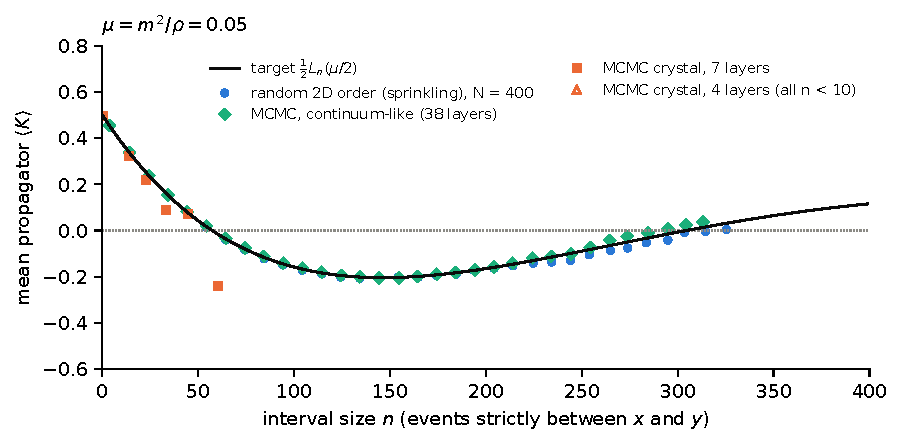
\includegraphics[width=\columnwidth]{fig_laguerre}
%DIFDELCMD < %%%
\DIFdelendFL \DIFaddbeginFL 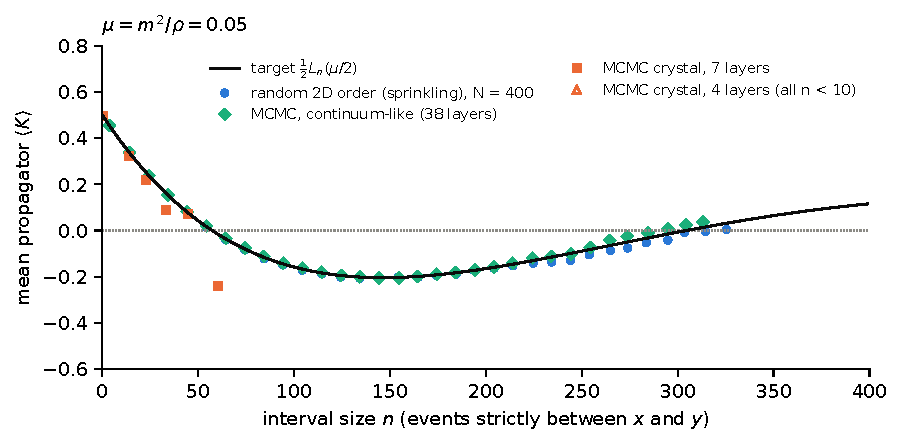
\includegraphics[width=0.6\textwidth]{fig_laguerre}
\DIFaddendFL \caption{Johnston's propagator averaged over related pairs with interval size $n$, against $\tfrac12L_n(\mu/2)$, at $\mu=0.05$ and $N=400$. At large $n$ few pairs remain and the bins are noisy. In the 4-layer crystal every interval has fewer than 10 elements, so it contributes a single point near $n=0$.}
\label{fig:laguerre}
\end{figure}

\section{Other approaches tested}\label{app:dropped}
\begin{itemize}
\item \emph{Fixed-$n$ propagator as a curvature estimator.} In curved $1+1$ spacetime a term $(R\tau^2/48)J_2(m\tau)$ appears in the propagator~\cite{NXDS17}. In a de Sitter diamond conditioned on $n$ elements\DIFaddbegin \DIFadd{, }\DIFaddend the order depends only on $(n,H\tau)$, so a fixed-$n$ curvature test exists. We find that the fraction of related pairs rises by $\approx0.027\,(H\tau)^2$ for $n=10$--$60$, and that the fixed-$n$ propagator is no more sensitive than that fraction alone: a $3\sigma$ detection at $n=30$, $H\tau=1$ requires 175 intervals in either case. The fixed-$n$ propagator therefore detects curvature only through the known chain-abundance route~\cite{RSS13}.
\item \emph{Embedding test on small orders.} We first applied the test to exhaustive ensembles of small orders ($N\leq12$). \DIFdelbegin \DIFdel{Its }\DIFdelend \DIFaddbegin \DIFadd{At these sizes its }\DIFaddend statistics do not separate flat from layered orders\DIFdelbegin \DIFdel{at these sizes, and only settle }\DIFdelend \DIFaddbegin \DIFadd{; they settle only }\DIFaddend for $N\gtrsim100$ [\DIFdelbegin \DIFdel{Fig.}\DIFdelend \DIFaddbegin \DIFadd{figure}\DIFaddend ~\ref{fig:detector}(a)], so we moved to Monte Carlo samples at $N\geq200$.
\item \emph{Hysteresis in the \DIFdelbegin \DIFdel{$e^{-\beta S}$ }\DIFdelend \DIFaddbegin \DIFadd{$\rme^{-\beta S}$ }\DIFaddend chains.} At $N=400$, chains started from random and from layered orders at the same $\beta$ end in different phases. We first read this as hysteresis of the transition\DIFdelbegin \DIFdel{; }\DIFdelend \DIFaddbegin \DIFadd{. However, }\DIFaddend the chains from layered starts accept $\leq0.1\%$ of the moves and are effectively frozen, so the difference reflects the sampler rather than the model.
\item \emph{Two-dimensional estimator on $2+1$ sprinklings.} Fed into the embedding, \DIFdelbegin \DIFdel{Eq.~\eqref{eq:est} }\DIFdelend \DIFaddbegin \DIFadd{equation~}\eref{eq:est} \DIFaddend applied to a $2+1$ sprinkling (with the $2+1$ density) produces two large positive eigenvalues. The formula is not valid there, so this is at most a qualitative indication that the spectrum counts spatial dimensions.
\end{itemize}

\DIFaddbegin \section*{\DIFadd{References}}
\DIFaddend \begin{thebibliography}{99}
\bibitem{BLMS87} \DIFdelbegin \DIFdel{L.~Bombelli , J.~Lee , D.~Meyer , and R.~D .~Sorkin, }\DIFdelend \DIFaddbegin \DIFadd{Bombelli L, Lee J, Meyer D and Sorkin R D 1987 }\DIFaddend Space-time as a causal set \DIFdelbegin \DIFdel{, Phys. \ Rev. \ Lett.\ }\textbf{\DIFdel{59}}%DIFAUXCMD
\DIFdel{, }\DIFdelend \DIFaddbegin {\it \DIFadd{Phys. Rev. Lett.}} {\bf \DIFadd{59}} \DIFaddend 521
\DIFdelbegin \DIFdel{(1987).
}\DIFdelend \bibitem{Surya19} \DIFdelbegin \DIFdel{S.~Surya , }\DIFdelend \DIFaddbegin \DIFadd{Surya S 2019 }\DIFaddend The causal set approach to quantum gravity \DIFdelbegin \DIFdel{, }\DIFdelend \DIFaddbegin {\it \DIFaddend Living Rev. \DIFdelbegin \DIFdel{\ Relativ.\ }\textbf{\DIFdel{22}}%DIFAUXCMD
\DIFdel{, }\DIFdelend \DIFaddbegin \DIFadd{Relativ.}} {\bf \DIFadd{22}} \DIFaddend 5 (\DIFdelbegin \DIFdel{2019), }\DIFdelend arXiv:1903.11544\DIFdelbegin \DIFdel{.
}\DIFdelend \DIFaddbegin \DIFadd{)
}\DIFaddend \bibitem{BrightwellGregory91} \DIFdelbegin \DIFdel{G.~Brightwell and R.~Gregory , }\DIFdelend \DIFaddbegin \DIFadd{Brightwell G and Gregory R 1991 }\DIFaddend Structure of random discrete spacetime \DIFdelbegin \DIFdel{, Phys. \ Rev. \ Lett.\ }\textbf{\DIFdel{66}}%DIFAUXCMD
\DIFdel{, }\DIFdelend \DIFaddbegin {\it \DIFadd{Phys. Rev. Lett.}} {\bf \DIFadd{66}} \DIFaddend 260
\DIFdelbegin \DIFdel{(1991).
}\DIFdelend \bibitem{Myrheim78} \DIFdelbegin \DIFdel{J.~Myrheim , Statistical geometry , CERN ReportNo.\ }\DIFdelend \DIFaddbegin \DIFadd{Myrheim J 1978 Statistical geometry }{\it \DIFadd{CERN Report}} \DIFaddend TH-2538
\DIFdelbegin \DIFdel{, 1978.
}\DIFdelend \bibitem{Meyer88} \DIFdelbegin \DIFdel{D.~A .~Meyer, }\DIFdelend \DIFaddbegin \DIFadd{Meyer D A 1988 }\DIFaddend The dimension of causal sets \DIFdelbegin \DIFdel{, Ph.D.\ thesis, }\DIFdelend \DIFaddbegin {\it \DIFadd{PhD Thesis}} \DIFaddend Massachusetts Institute of Technology
\DIFdelbegin \DIFdel{, 1988.
}\DIFdelend \bibitem{RSS13} \DIFdelbegin \DIFdel{M.~Roy , D.~Sinha , and S.~Surya , }\DIFdelend \DIFaddbegin \DIFadd{Roy M, Sinha D and Surya S 2013 }\DIFaddend Discrete geometry of a small causal diamond \DIFdelbegin \DIFdel{, Phys. \ Rev.\ D }\textbf{\DIFdel{87}}%DIFAUXCMD
\DIFdel{, }\DIFdelend \DIFaddbegin {\it \DIFadd{Phys. Rev.}} \DIFadd{D }{\bf \DIFadd{87}} \DIFaddend 044046 (\DIFdelbegin \DIFdel{2013), }\DIFdelend arXiv:1212.0631\DIFdelbegin \DIFdel{.
}\DIFdelend \DIFaddbegin \DIFadd{)
}\DIFaddend \bibitem{GlaserSurya13} \DIFdelbegin \DIFdel{L.~Glaser and S.~Surya , }\DIFdelend \DIFaddbegin \DIFadd{Glaser L and Surya S 2013 }\DIFaddend Towards a definition of locality in a manifoldlike causal set \DIFdelbegin \DIFdel{, Phys. \ Rev.\ D }\textbf{\DIFdel{88}}%DIFAUXCMD
\DIFdel{, }\DIFdelend \DIFaddbegin {\it \DIFadd{Phys. Rev.}} \DIFadd{D }{\bf \DIFadd{88}} \DIFaddend 124026 (\DIFdelbegin \DIFdel{2013), }\DIFdelend arXiv:1309.3403\DIFdelbegin \DIFdel{.
}\DIFdelend \DIFaddbegin \DIFadd{)
}\DIFaddend \bibitem{BD10} \DIFdelbegin \DIFdel{D.~M .~T .~Benincasa and F.~Dowker , }\DIFdelend \DIFaddbegin \DIFadd{Benincasa D M T and Dowker F 2010 }\DIFaddend The scalar curvature of a causal set \DIFdelbegin \DIFdel{, Phys. \ Rev. \ Lett.\ }\textbf{\DIFdel{104}}%DIFAUXCMD
\DIFdel{, }\DIFdelend \DIFaddbegin {\it \DIFadd{Phys. Rev. Lett.}} {\bf \DIFadd{104}} \DIFaddend 181301 (\DIFdelbegin \DIFdel{2010), }\DIFdelend arXiv:1001.2725\DIFdelbegin \DIFdel{.
}\DIFdelend \DIFaddbegin \DIFadd{)
}\DIFaddend \bibitem{DowkerGlaser13} \DIFdelbegin \DIFdel{F.~Dowker and L.~Glaser , }\DIFdelend \DIFaddbegin \DIFadd{Dowker F and Glaser L 2013 }\DIFaddend Causal set d'Alembertians for various dimensions \DIFdelbegin \DIFdel{, Classical Quantum Gravity }\textbf{\DIFdel{30}}%DIFAUXCMD
\DIFdel{, }\DIFdelend \DIFaddbegin {\it \DIFadd{Class. Quantum Grav.}} {\bf \DIFadd{30}} \DIFaddend 195016 (\DIFdelbegin \DIFdel{2013), }\DIFdelend arXiv:1305.2588\DIFdelbegin \DIFdel{.
}\DIFdelend \DIFaddbegin \DIFadd{)
}\DIFaddend \bibitem{BK24} \DIFdelbegin \DIFdel{M.~}\DIFdelend Bogu\~n\'a \DIFdelbegin \DIFdel{and D.~Krioukov , }\DIFdelend \DIFaddbegin \DIFadd{M and Krioukov D 2024 }\DIFaddend Measuring spatial distances in causal sets via causal overlaps \DIFdelbegin \DIFdel{, Phys. \ Rev.\ D }\textbf{\DIFdel{110}}%DIFAUXCMD
\DIFdel{, }\DIFdelend \DIFaddbegin {\it \DIFadd{Phys. Rev.}} \DIFadd{D }{\bf \DIFadd{110}} \DIFaddend 024008 (\DIFdelbegin \DIFdel{2024), }\DIFdelend arXiv:2401.17376\DIFdelbegin \DIFdel{.
}\DIFdelend \DIFaddbegin \DIFadd{)
}\DIFaddend \bibitem{RideoutWallden09} \DIFdelbegin \DIFdel{D.~Rideout and P.~Wallden , }\DIFdelend \DIFaddbegin \DIFadd{Rideout D and Wallden P 2009 }\DIFaddend Spacelike distance from discrete causal order \DIFdelbegin \DIFdel{, Classical Quantum Gravity }\textbf{\DIFdel{26}}%DIFAUXCMD
\DIFdel{, }\DIFdelend \DIFaddbegin {\it \DIFadd{Class. Quantum Grav.}} {\bf \DIFadd{26}} \DIFaddend 155013 (\DIFdelbegin \DIFdel{2009), }\DIFdelend arXiv:0810.1768\DIFdelbegin \DIFdel{.
}\DIFdelend \DIFaddbegin \DIFadd{)
}\DIFaddend \bibitem{MRS06} \DIFdelbegin \DIFdel{S.~Major , D.~Rideout , and S.~Surya , }\DIFdelend \DIFaddbegin \DIFadd{Major S, Rideout D and Surya S 2006 }\DIFaddend Spatial hypersurfaces in causal set cosmology \DIFdelbegin \DIFdel{, Classical Quantum Gravity }\textbf{\DIFdel{23}}%DIFAUXCMD
\DIFdel{, }\DIFdelend \DIFaddbegin {\it \DIFadd{Class. Quantum Grav.}} {\bf \DIFadd{23}} \DIFaddend 4743 (\DIFdelbegin \DIFdel{2006), }\DIFdelend arXiv:gr-qc/\DIFdelbegin \DIFdel{0506133.
}\DIFdelend \DIFaddbegin \DIFadd{0506133)
}\DIFaddend \bibitem{MRS07} \DIFdelbegin \DIFdel{S.~Major , D.~Rideout , and S.~Surya , }\DIFdelend \DIFaddbegin \DIFadd{Major S, Rideout D and Surya S 2007 }\DIFaddend On recovering continuum topology from a causal set \DIFdelbegin \DIFdel{, J. \ Math. \ Phys.\ }\textbf{\DIFdel{48}}%DIFAUXCMD
\DIFdel{, }\DIFdelend \DIFaddbegin {\it \DIFadd{J. Math. Phys.}} {\bf \DIFadd{48}} \DIFaddend 032501 (\DIFdelbegin \DIFdel{2007), }\DIFdelend arXiv:gr-qc/\DIFdelbegin \DIFdel{0604124.
}\DIFdelend \DIFaddbegin \DIFadd{0604124)
}\DIFaddend \bibitem{ESV19} \DIFdelbegin \DIFdel{A.~Eichhorn , S.~Surya , and F.~Versteegen , }\DIFdelend \DIFaddbegin \DIFadd{Eichhorn A, Surya S and Versteegen F 2019 }\DIFaddend Induced spatial geometry from causal structure \DIFdelbegin \DIFdel{, Classical Quantum Gravity }\textbf{\DIFdel{36}}%DIFAUXCMD
\DIFdel{, }\DIFdelend \DIFaddbegin {\it \DIFadd{Class. Quantum Grav.}} {\bf \DIFadd{36}} \DIFaddend 105005 (\DIFdelbegin \DIFdel{2019), }\DIFdelend arXiv:1809.06192\DIFdelbegin \DIFdel{.
}\DIFdelend \DIFaddbegin \DIFadd{)
}\DIFaddend \bibitem{KhetrapalSurya13} \DIFdelbegin \DIFdel{S.~Khetrapal and S .~Surya , }\DIFdelend \DIFaddbegin \DIFadd{Khetrapal S and Surya S 2013 }\DIFaddend Boundary term contribution to the volume of a small causal diamond \DIFdelbegin \DIFdel{, Classical Quantum Gravity }\textbf{\DIFdel{30}}%DIFAUXCMD
\DIFdel{, }\DIFdelend \DIFaddbegin {\it \DIFadd{Class. Quantum Grav.}} {\bf \DIFadd{30}} \DIFaddend 065005 (\DIFdelbegin \DIFdel{2013), }\DIFdelend arXiv:1212.0629\DIFdelbegin \DIFdel{.
}\DIFdelend \DIFaddbegin \DIFadd{)
}\DIFaddend \bibitem{GlaserSurya16} \DIFdelbegin \DIFdel{L.~Glaser and S.~Surya , }\DIFdelend \DIFaddbegin \DIFadd{Glaser L and Surya S 2016 }\DIFaddend The Hartle--Hawking wave function in 2D causal set quantum gravity \DIFdelbegin \DIFdel{, Classical Quantum Gravity }\textbf{\DIFdel{33}}%DIFAUXCMD
\DIFdel{, }\DIFdelend \DIFaddbegin {\it \DIFadd{Class. Quantum Grav.}} {\bf \DIFadd{33}} \DIFaddend 065003 (\DIFdelbegin \DIFdel{2016), }\DIFdelend arXiv:1410.8775\DIFdelbegin \DIFdel{.
}\DIFdelend \DIFaddbegin \DIFadd{)
}\DIFaddend \bibitem{Glaser18} \DIFdelbegin \DIFdel{L.~Glaser , }\DIFdelend \DIFaddbegin \DIFadd{Glaser L 2018 }\DIFaddend The Ising model coupled to 2d orders \DIFdelbegin \DIFdel{, Classical Quantum Gravity }\textbf{\DIFdel{35}}%DIFAUXCMD
\DIFdel{, }\DIFdelend \DIFaddbegin {\it \DIFadd{Class. Quantum Grav.}} {\bf \DIFadd{35}} \DIFaddend 084001 (\DIFdelbegin \DIFdel{2018), }\DIFdelend arXiv:1802.02519\DIFdelbegin \DIFdel{.
}\DIFdelend \DIFaddbegin \DIFadd{)
}\DIFaddend \bibitem{Glaser23} \DIFdelbegin \DIFdel{L.~Glaser , }\DIFdelend \DIFaddbegin \DIFadd{Glaser L 2023 }\DIFaddend Computer simulations of causal sets \DIFdelbegin \DIFdel{, }\DIFdelend arXiv:2306.09904
\DIFdelbegin \DIFdel{(2023).
}\DIFdelend \bibitem{HMM25} \DIFdelbegin \DIFdel{C.~A.~Hu, D.~A .~Meyer, and E.~J .~Q .~Meyer, }\DIFdelend \DIFaddbegin \DIFadd{Hu C A, Meyer D A and Meyer E J Q 2025 }\DIFaddend Reconstructing Minkowski geometry from causal separations \DIFdelbegin \DIFdel{, J. \ Math. \ Phys.\ }\textbf{\DIFdel{66}}%DIFAUXCMD
\DIFdel{, }\DIFdelend \DIFaddbegin {\it \DIFadd{J. Math. Phys.}} {\bf \DIFadd{66}} \DIFaddend 122502 (\DIFdelbegin \DIFdel{2025), }\DIFdelend arXiv:2601.03280\DIFdelbegin \DIFdel{.
}\DIFdelend \DIFaddbegin \DIFadd{)
}\DIFaddend \bibitem{CloughEvans16} \DIFdelbegin \DIFdel{J.~R .~Clough and T.~S .~Evans, }\DIFdelend \DIFaddbegin \DIFadd{Clough J R and Evans T S 2017 }\DIFaddend Embedding graphs in Lorentzian spacetime \DIFdelbegin \DIFdel{, PLoS One}\textbf{\DIFdel{12}}%DIFAUXCMD
\DIFdel{, }\DIFdelend \DIFaddbegin {\it \DIFadd{PLoS One}} {\bf \DIFadd{12}} \DIFaddend e0187301 (\DIFdelbegin \DIFdel{2017), }\DIFdelend arXiv:1602.03103\DIFdelbegin \DIFdel{.
}\DIFdelend \DIFaddbegin \DIFadd{)
}\DIFaddend \bibitem{Clough17} \DIFdelbegin \DIFdel{J.~R .~Clough, }\DIFdelend \DIFaddbegin \DIFadd{Clough J R 2017 }\DIFaddend Causal structure in networks \DIFdelbegin \DIFdel{, Ph.D.\ thesis, }\DIFdelend \DIFaddbegin {\it \DIFadd{PhD Thesis}} \DIFaddend Imperial College London \DIFdelbegin \DIFdel{, 2017, }\DIFdelend \DIFaddbegin \DIFadd{(}\DIFaddend hdl:10044/1/\DIFdelbegin \DIFdel{50162.
}\DIFdelend \DIFaddbegin \DIFadd{50162)
}\DIFaddend \bibitem{Henson06} \DIFdelbegin \DIFdel{J.~Henson , }\DIFdelend \DIFaddbegin \DIFadd{Henson J 2006 }\DIFaddend Constructing an interval of Minkowski space from a causal set \DIFdelbegin \DIFdel{, Classical Quantum Gravity }\textbf{\DIFdel{23}}%DIFAUXCMD
\DIFdel{, }\DIFdelend \DIFaddbegin {\it \DIFadd{Class. Quantum Grav.}} {\bf \DIFadd{23}} \DIFaddend L29 (\DIFdelbegin \DIFdel{2006), }\DIFdelend arXiv:gr-qc/\DIFdelbegin \DIFdel{0601069.
}\DIFdelend \DIFaddbegin \DIFadd{0601069)
}\DIFaddend \bibitem{Johnston25} \DIFdelbegin \DIFdel{S.~Johnston , }\DIFdelend \DIFaddbegin \DIFadd{Johnston S 2025 }\DIFaddend Simpler embeddings of causal sets into Minkowski spacetime \DIFdelbegin \DIFdel{, Phys. \ Rev.\ D }\textbf{\DIFdel{111}}%DIFAUXCMD
\DIFdel{, }\DIFdelend \DIFaddbegin {\it \DIFadd{Phys. Rev.}} \DIFadd{D }{\bf \DIFadd{111}} \DIFaddend 106020 (\DIFdelbegin \DIFdel{2025), }\DIFdelend arXiv:2502.09701\DIFdelbegin \DIFdel{.
}\DIFdelend \DIFaddbegin \DIFadd{)
}\DIFaddend \bibitem{Johnston08} \DIFdelbegin \DIFdel{S.~Johnston , }\DIFdelend \DIFaddbegin \DIFadd{Johnston S 2008 }\DIFaddend Particle propagators on discrete spacetime \DIFdelbegin \DIFdel{, Classical Quantum Gravity }\textbf{\DIFdel{25}}%DIFAUXCMD
\DIFdel{, }\DIFdelend \DIFaddbegin {\it \DIFadd{Class. Quantum Grav.}} {\bf \DIFadd{25}} \DIFaddend 202001 (\DIFdelbegin \DIFdel{2008), }\DIFdelend arXiv:0806.3083\DIFdelbegin \DIFdel{.
}\DIFdelend \DIFaddbegin \DIFadd{)
}\DIFaddend \bibitem{Johnston09} \DIFdelbegin \DIFdel{S.~Johnston , }\DIFdelend \DIFaddbegin \DIFadd{Johnston S 2009 }\DIFaddend Feynman propagator for a free scalar field on a causal set \DIFdelbegin \DIFdel{, Phys. \ Rev. \ Lett.\ }\textbf{\DIFdel{103}}%DIFAUXCMD
\DIFdel{, }\DIFdelend \DIFaddbegin {\it \DIFadd{Phys. Rev. Lett.}} {\bf \DIFadd{103}} \DIFaddend 180401 (\DIFdelbegin \DIFdel{2009), }\DIFdelend arXiv:0909.0944\DIFdelbegin \DIFdel{.
}\DIFdelend \DIFaddbegin \DIFadd{)
}\DIFaddend \bibitem{BHS08} \DIFdelbegin \DIFdel{G.~Brightwell , J.~Henson , and S.~Surya , }\DIFdelend \DIFaddbegin \DIFadd{Brightwell G, Henson J and Surya S 2008 }\DIFaddend A 2D model of causal set quantum gravity: the emergence of the continuum \DIFdelbegin \DIFdel{, Classical Quantum Gravity }\textbf{\DIFdel{25}}%DIFAUXCMD
\DIFdel{, }\DIFdelend \DIFaddbegin {\it \DIFadd{Class. Quantum Grav.}} {\bf \DIFadd{25}} \DIFaddend 105025 (\DIFdelbegin \DIFdel{2008), }\DIFdelend arXiv:0706.0375\DIFdelbegin \DIFdel{.
}\DIFdelend \DIFaddbegin \DIFadd{)
}\DIFaddend \bibitem{Surya12} \DIFdelbegin \DIFdel{S.~Surya , }\DIFdelend \DIFaddbegin \DIFadd{Surya S 2012 }\DIFaddend Evidence for the continuum in 2D causal set quantum gravity \DIFdelbegin \DIFdel{, Classical Quantum Gravity }\textbf{\DIFdel{29}}%DIFAUXCMD
\DIFdel{, }\DIFdelend \DIFaddbegin {\it \DIFadd{Class. Quantum Grav.}} {\bf \DIFadd{29}} \DIFaddend 132001 (\DIFdelbegin \DIFdel{2012), }\DIFdelend arXiv:1110.6244\DIFdelbegin \DIFdel{.
}\DIFdelend \DIFaddbegin \DIFadd{)
}\DIFaddend \bibitem{GOS18} \DIFdelbegin \DIFdel{L.~Glaser , D.~}\DIFdelend \DIFaddbegin \DIFadd{Glaser L, }\DIFaddend O'Connor \DIFdelbegin \DIFdel{, and S.~Surya , }\DIFdelend \DIFaddbegin \DIFadd{D and Surya S 2018 }\DIFaddend Finite size scaling in 2d causal set quantum gravity \DIFdelbegin \DIFdel{, Classical Quantum Gravity }\textbf{\DIFdel{35}}%DIFAUXCMD
\DIFdel{, }\DIFdelend \DIFaddbegin {\it \DIFadd{Class. Quantum Grav.}} {\bf \DIFadd{35}} \DIFaddend 045006 (\DIFdelbegin \DIFdel{2018), }\DIFdelend arXiv:1706.06432\DIFdelbegin \DIFdel{.
}\DIFdelend \DIFaddbegin \DIFadd{)
}\DIFaddend \bibitem{Embedding} \DIFdelbegin \DIFdel{R.~Bada , }\DIFdelend \DIFaddbegin \DIFadd{Bada R 2026 }\DIFaddend Spatial embedding of $3+1$ causal sets: low-count spacelike pairs and a likelihood fit to interval counts (companion paper, \DIFdelbegin \DIFdel{2026), }\DIFdelend to be submitted\DIFdelbegin \DIFdel{.
}\DIFdelend \DIFaddbegin \DIFadd{)
}\DIFaddend \bibitem{BDJ99} \DIFdelbegin \DIFdel{J.~Baik , P.~Deift , and K.~Johansson , }\DIFdelend \DIFaddbegin \DIFadd{Baik J, Deift P and Johansson K 1999 }\DIFaddend On the distribution of the length of the longest increasing subsequence of random permutations \DIFdelbegin \DIFdel{, J. \ Am. \ Math. \ Soc.\ }\textbf{\DIFdel{12}}%DIFAUXCMD
\DIFdel{, }\DIFdelend \DIFaddbegin {\it \DIFadd{J. Am. Math. Soc.}} {\bf \DIFadd{12}} \DIFaddend 1119
\DIFdelbegin \DIFdel{(1999).
}\DIFdelend \bibitem{Cunningham18} \DIFdelbegin \DIFdel{W.~J .~Cunningham, }\DIFdelend \DIFaddbegin \DIFadd{Cunningham W J 2018 }\DIFaddend Inference of boundaries in causal sets \DIFdelbegin \DIFdel{, Classical Quantum Gravity }\textbf{\DIFdel{35}}%DIFAUXCMD
\DIFdel{, }\DIFdelend \DIFaddbegin {\it \DIFadd{Class. Quantum Grav.}} {\bf \DIFadd{35}} \DIFaddend 094002 (\DIFdelbegin \DIFdel{2018), }\DIFdelend arXiv:1710.09705\DIFdelbegin \DIFdel{.
}\DIFdelend \DIFaddbegin \DIFadd{)
}\DIFaddend \bibitem{BBR26} \DIFdelbegin \DIFdel{J.~Barton , S.~Borza , and J.~}\DIFdelend \DIFaddbegin \DIFadd{Barton J, Borza S and }\DIFaddend R\"ohrig \DIFdelbegin \DIFdel{, }\DIFdelend \DIFaddbegin \DIFadd{J 2026 }\DIFaddend Ollivier--Ricci curvature for causal sets \DIFdelbegin \DIFdel{, }\DIFdelend arXiv:2606.04910
\DIFdelbegin \DIFdel{(2026).
}\DIFdelend \bibitem{LastPenrose17} \DIFdelbegin \DIFdel{G.~Last and M.~Penrose , }\emph{\DIFdel{Lectures on the Poisson Process}} %DIFAUXCMD
\DIFdel{(CambridgeUniversity Press, Cambridge, 2017) , Ch.~4.
}\DIFdelend \DIFaddbegin \DIFadd{Last G and Penrose M 2017 }{\it \DIFadd{Lectures on the Poisson Process}} \DIFadd{(Cambridge: Cambridge University Press) ch~4
}\DIFaddend \bibitem{Pinsky06} \DIFdelbegin \DIFdel{R.~G .~Pinsky, }\DIFdelend \DIFaddbegin \DIFadd{Pinsky R G 2006 }\DIFaddend Law of large numbers for increasing subsequences of random permutations \DIFdelbegin \DIFdel{, }\DIFdelend \DIFaddbegin {\it \DIFaddend Random Struct. \DIFdelbegin \DIFdel{\ Algorithms}\textbf{\DIFdel{29}}%DIFAUXCMD
\DIFdel{, }\DIFdelend \DIFaddbegin \DIFadd{Algorithms}} {\bf \DIFadd{29}} \DIFaddend 277 (\DIFdelbegin \DIFdel{2006), }\DIFdelend arXiv:math/0407353\DIFdelbegin \DIFdel{, Eq.}\DIFdelend \DIFaddbegin \DIFadd{) equation}\DIFaddend ~(1.1)
\DIFdelbegin \DIFdel{.
}\DIFdelend \bibitem{Szego39} \DIFdelbegin \DIFdel{G.~Szeg\H{o} , }\emph{\DIFdel{Orthogonal Polynomials}}%DIFAUXCMD
\DIFdel{, }\DIFdelend \DIFaddbegin \DIFadd{Szeg\H{o} G 1939 }{\it \DIFadd{Orthogonal Polynomials}} \DIFadd{(}\DIFaddend American Mathematical Society Colloquium Publications \DIFdelbegin \DIFdel{Vol.}\DIFdelend \DIFaddbegin \DIFadd{vol}\DIFaddend ~23\DIFdelbegin \DIFdel{(AMS, New York, 1939)
.
}\DIFdelend \DIFaddbegin \DIFadd{) (New York: American Mathematical Society)
}\DIFaddend \bibitem{LifschitzPittel81} \DIFdelbegin \DIFdel{V.~Lifschitz and B.~Pittel , }\DIFdelend \DIFaddbegin \DIFadd{Lifschitz V and Pittel B 1981 }\DIFaddend The number of increasing subsequences of the random permutation \DIFdelbegin \DIFdel{, J. \ Comb. \ TheorySer.\ A }\textbf{\DIFdel{31}}%DIFAUXCMD
\DIFdel{, }\DIFdelend \DIFaddbegin {\it \DIFadd{J. Comb. Theory}} \DIFadd{A }{\bf \DIFadd{31}} \DIFaddend 1
\DIFdelbegin \DIFdel{(1981).
}\DIFdelend \bibitem{OEIS} OEIS Foundation \DIFdelbegin \DIFdel{, }\DIFdelend The On-Line Encyclopedia of Integer Sequences, sequence A002720 \DIFdelbegin \DIFdel{, }\DIFdelend \url{https://oeis.org/A002720}
\DIFdelbegin \DIFdel{.
}\DIFdelend \bibitem{ABP18} \DIFdelbegin \DIFdel{M.~E.~Aghili, L.~Bombelli , and }\DIFdelend \DIFaddbegin \DIFadd{Aghili M E, Bombelli L and Pilgrim B }\DIFaddend B \DIFdelbegin \DIFdel{.~B .~Pilgrim, }\DIFdelend \DIFaddbegin \DIFadd{2018 }\DIFaddend Path length distribution in two-dimensional causal sets \DIFdelbegin \DIFdel{, Eur. \ Phys. \ J.\ C }\textbf{\DIFdel{78}}%DIFAUXCMD
\DIFdel{, }\DIFdelend \DIFaddbegin {\it \DIFadd{Eur. Phys. J.}} \DIFadd{C }{\bf \DIFadd{78}} \DIFaddend 744 (\DIFdelbegin \DIFdel{2018), }\DIFdelend arXiv:1805.07312\DIFdelbegin \DIFdel{.
}\DIFdelend \DIFaddbegin \DIFadd{)
}\DIFaddend \bibitem{Shuman23} \DIFdelbegin \DIFdel{S.~Shuman , }\DIFdelend \DIFaddbegin \DIFadd{Shuman S 2024 }\DIFaddend Path sums for propagators in causal sets \DIFdelbegin \DIFdel{, Phys. \ Rev.\ D }\textbf{\DIFdel{109}}%DIFAUXCMD
\DIFdel{, }\DIFdelend \DIFaddbegin {\it \DIFadd{Phys. Rev.}} \DIFadd{D }{\bf \DIFadd{109}} \DIFaddend 046008 (\DIFdelbegin \DIFdel{2024), }\DIFdelend arXiv:2307.08864\DIFdelbegin \DIFdel{.
}\DIFdelend \DIFaddbegin \DIFadd{)
}\DIFaddend \bibitem{KastratiHinrichsen26} \DIFdelbegin \DIFdel{A.~Kastrati and H.~Hinrichsen , }\DIFdelend \DIFaddbegin \DIFadd{Kastrati A and Hinrichsen H 2026 }\DIFaddend Numerical evaluation of the causal set propagator in 2D anti-de Sitter spacetime \DIFdelbegin \DIFdel{, Phys. \ Rev.\ D }\textbf{\DIFdel{113}}%DIFAUXCMD
\DIFdel{, }\DIFdelend \DIFaddbegin {\it \DIFadd{Phys. Rev.}} \DIFadd{D }{\bf \DIFadd{113}} \DIFaddend 065003 (\DIFdelbegin \DIFdel{2026), }\DIFdelend arXiv:2504.12919\DIFdelbegin \DIFdel{.
}\DIFdelend \DIFaddbegin \DIFadd{)
}\DIFaddend \bibitem{EMLW26} \DIFdelbegin \DIFdel{A.~Eichhorn , H.~Mack , K.~T .~Le, and F.~Wagner , }\DIFdelend \DIFaddbegin \DIFadd{Eichhorn A, Mack H, Le K T and Wagner F 2026 }\DIFaddend Charting causal set configuration space with graph observables \DIFdelbegin \DIFdel{, }\DIFdelend arXiv:2605.27514
\DIFdelbegin \DIFdel{(2026).
}\DIFdelend \bibitem{RideoutSorkin00} \DIFaddbegin \DIFadd{Rideout D P and Sorkin R }\DIFaddend D \DIFdelbegin \DIFdel{.~P .~Rideout and R.~D .~Sorkin, }\DIFdelend \DIFaddbegin \DIFadd{2000 }\DIFaddend Classical sequential growth dynamics for causal sets \DIFdelbegin \DIFdel{, Phys. \ Rev.\ D }\textbf{\DIFdel{61}}%DIFAUXCMD
\DIFdel{, }\DIFdelend \DIFaddbegin {\it \DIFadd{Phys. Rev.}} \DIFadd{D }{\bf \DIFadd{61}} \DIFaddend 024002
\DIFdelbegin \DIFdel{(2000).
}\DIFdelend \bibitem{MORS01} \DIFdelbegin \DIFdel{X.~}\DIFdelend Mart\'in \DIFdelbegin \DIFdel{, D.~}\DIFdelend \DIFaddbegin \DIFadd{X, }\DIFaddend O'Connor \DIFdelbegin \DIFdel{, }\DIFdelend \DIFaddbegin \DIFadd{D, Rideout D P and Sorkin R }\DIFaddend D \DIFdelbegin \DIFdel{.~P .~Rideout, and R.~D .~Sorkin, }\DIFdelend \DIFaddbegin \DIFadd{2001 }\DIFaddend On the renormalization transformations induced by cycles of expansion and contraction in causal set cosmology \DIFdelbegin \DIFdel{, Phys. \ Rev.\ D }\textbf{\DIFdel{63}}%DIFAUXCMD
\DIFdel{, }\DIFdelend \DIFaddbegin {\it \DIFadd{Phys. Rev.}} \DIFadd{D }{\bf \DIFadd{63}} \DIFaddend 084026
\DIFdelbegin \DIFdel{(2001).
}\DIFdelend \bibitem{AhmedRideout10} \DIFdelbegin \DIFdel{M.~Ahmed and D.~Rideout , }\DIFdelend \DIFaddbegin \DIFadd{Ahmed M and Rideout D 2010 }\DIFaddend Indications of de Sitter spacetime from classical sequential growth dynamics of causal sets \DIFdelbegin \DIFdel{, Phys. \ Rev.\ D }\textbf{\DIFdel{81}}%DIFAUXCMD
\DIFdel{, }\DIFdelend \DIFaddbegin {\it \DIFadd{Phys. Rev.}} \DIFadd{D }{\bf \DIFadd{81}} \DIFaddend 083528
\DIFdelbegin \DIFdel{(2010).
}\DIFdelend \bibitem{CunninghamSurya19} \DIFdelbegin \DIFdel{W.~J .~Cunningham and S.~Surya , }\DIFdelend \DIFaddbegin \DIFadd{Cunningham W J and Surya S 2020 }\DIFaddend Dimensionally restricted causal set quantum gravity: examples in two and three dimensions \DIFdelbegin \DIFdel{, Classical Quantum Gravity }\textbf{\DIFdel{37}}%DIFAUXCMD
\DIFdel{, }\DIFdelend \DIFaddbegin {\it \DIFadd{Class. Quantum Grav.}} {\bf \DIFadd{37}} \DIFaddend 054002 (\DIFdelbegin \DIFdel{2020), }\DIFdelend arXiv:1908.11647\DIFdelbegin \DIFdel{.
}\DIFdelend \DIFaddbegin \DIFadd{)
}\DIFaddend \bibitem{NXDS17} Nomaan \DIFdelbegin \DIFdel{~X, F.~Dowker , and S.~Surya }\DIFdelend \DIFaddbegin \DIFadd{X}\DIFaddend , \DIFaddbegin \DIFadd{Dowker F and Surya S 2017 }\DIFaddend Scalar field Green functions on causal sets \DIFdelbegin \DIFdel{, Classical Quantum Gravity }\textbf{\DIFdel{34}}%DIFAUXCMD
\DIFdel{, }\DIFdelend \DIFaddbegin {\it \DIFadd{Class. Quantum Grav.}} {\bf \DIFadd{34}} \DIFaddend 124002 (\DIFdelbegin \DIFdel{2017), }\DIFdelend arXiv:1701.07212\DIFdelbegin \DIFdel{.
}\DIFdelend \DIFaddbegin \DIFadd{)
}\DIFaddend \bibitem{MethodNote} \DIFdelbegin \DIFdel{R.~Bada , }\DIFdelend \DIFaddbegin \DIFadd{Bada R 2026 }\DIFaddend Two causal-set papers written with an AI research partner: methodology note\DIFdelbegin \DIFdel{(2026)}\DIFdelend , released with the code at \url{https://github.com/presindev/causet-counting}
\DIFdelbegin \DIFdel{.
}\DIFdelend \end{thebibliography}

\end{document}
